\documentclass[12pt,twoside,onecolumn,a4paper]{tesis}
\usepackage[T1]{fontenc}
\usepackage[latin1]{inputenc}
\usepackage[pdftex]{graphicx}
%\usepackage[small]{subfigure}
\usepackage{fancyheadings}
\usepackage{amsfonts}
\usepackage{amssymb}
\usepackage{multirow}
\usepackage{hyperref}
\usepackage{listings}

\pagestyle{fancy}
\bibliographystyle{unsrt}
\renewcommand{\chaptermark}[1]{\markboth{\chaptername\ \thechapter. #1}{}}
\renewcommand{\sectionmark}[1]{\markright{\thesection. #1}}
\renewcommand{\baselinestretch}{1.1}
\lhead[\fancyplain{}{\thepage}]{\fancyplain{}{\rightmark}}
\rhead[\fancyplain{}{\leftmark}]{\fancyplain{}{\thepage}}
\cfoot{}


\renewcommand{\theenumi}{\arabic{enumi}.}
\renewcommand{\theenumii}{\theenumi\arabic{enumii}.}
\renewcommand{\theenumiii}{\theenumii\arabic{enumiii}.}
\renewcommand{\labelenumi}{\theenumi}
\renewcommand{\labelenumii}{\theenumii}
\renewcommand{\labelenumiii}{\theenumiii}

\oddsidemargin=2.5 cm
\marginparwidth=4 cm
\linespread{1.3}

%funcion para compilar solo una parte. Un solo fichero.
%\includeonly{intro,grid}

%%ampliar margenes cabecera
\def\changemargin#1#2{\list{}{\rightmargin#2\leftmargin#1}\item[]}
\let\endchangemargin=\endlist


\begin{document}
\pagestyle{empty}
\begin{titlepage}
\begin{changemargin}{-2.8cm}{0cm}
\begin{center}

\begin{figure}[tbp]
\hspace*{-1.5cm}

\includegraphics[width=0.99\textwidth]{imagenes/00.pdf}
\end{figure}

{\large \bf{UNIVERSIDADE DA CORU\~NA}}

{\large \bf{SCHOOL OF INFORMATICS}}

\vspace{0.25cm}

\emph{Department of Electronics and Systems}

\vspace{1.25cm}

%FINAL THESIS - COMPUTER SCIENCE

%\vspace{1.0cm}

{\huge \bf{Assessment, Design and Implementation of a Private Cloud for MapReduce Applications}}

\vspace{1.5cm}

\begin{flushright}
\begin{tabular}{r r@{}}
\textbf{Author:} & Marcos Salgueiro Balsa \\
& \\
& Patricia Gonz\'alez G\'omez \\
\textbf{Tutoring:} & Tom\'as Fern\'andez Pena \\
& Jos\'e Carlos Cabaleiro Rodr\'iguez \\
& \\
\textbf{Date:} & A Coru\~na, junio de 2013
\end{tabular}
\end{flushright}

\end{center}
\end{changemargin}
\end{titlepage}

\cleardoublepage
\pagestyle{empty}
\section*{}

\begin{flushright}
\textit{Give a man a fish, and you'll feed him for a day.\\
Teach a man to fish, and you'll feed him for a lifetime}.\\
\textbf{Anne Isabella Thackeray Ritchie}

\vspace{0.5cm}

\textit{Great spirits have always encountered violent opposition from mediocre minds.}\\
\textbf{Albert Einsten}

\vspace{0.5cm}

\textit{The supreme art of war is to subdue the enemy without fighting.}\\
\textbf{Sun Tzu, \emph{The Art of War}}

\vspace{0.5cm}

\textit{[...] It takes these very simple-minded instructions -- ``Go fetch a number, add it to this number, put the result there, perceive if it's greater than this other number'' -- but executes them at a rate of, let's say, 1,000,000 per second. At 1,000,000 per second, the results appear to be magic.}\\
\textbf{Steven Paul Jobs}
\end{flushright}

\cleardoublepage
%\pagestyle{empty}
%\chapter*{Especificaci\'on}\label{sec:spec}

\begin{flushleft}
    \begin{tabular}{l l}
        \textbf{T\'itulo:} & Evaluaci\'on, dise\~no e implementaci\'on de un cloud privado\\
        & para aplicaciones MapReduce \\
        & \\
        \textbf{Clase:} & Proyecto de investigaci\'on y desarrollo \\
        & \\
        \textbf{Autor:} & Marcos Salgueiro Balsa \\
        & \\
        & Patricia Gonz\'alez G\'omez \\
        \textbf{Tutores:} & Tom\'as Fern\'andez Pena \\
        & Jos\'e Carlos Cabaleiro Rodr\'iguez \\
        & \\
        \textbf{Tribunal:} \\
        & \\
        \textbf{Fecha:} & A Coru\~na, junio de 2013 \\
        & \\
        \textbf{Calificaci\'on:}
    \end{tabular}
\end{flushleft}


%\cleardoublepage
\pagestyle{empty}
\chapter*{Summary}
\noindent The history of computation has seen how the unending evolution of technology has promoted changes in its ways and means. Today, \textit{tablets} and \textit{smartphones}, quantitatively inferior managing and memorizing numbers, camp freely in a global market saturated with options. The tendency is clear: users will get to use more than one device to access the Internet and will want to have all their data synchronized and at hand, all the time.

But that is only a part of the equation. At the other side of every service there lies a server that must deal with an ever increasing traffic volume, while it maintains response delivery within outstanding delay times --- low latency \emph{may} have helped the infant Google rise above the competition. If we also added that the idea of surrounding every implementation effort with energetic efficiency is a transcendental requisite and not simply a good practice, we would have the perfect setup for the proliferation of new distributed paradigms like \emph{Cloud Computing}. Cloud Computing --- or just \emph{the cloud} --- is not intrinsically a new idea but an abstraction of an old idea: \emph{Virtualization}. The clouds' cornerstone is flexibility in providing a client with computational infrastructure.

Another technology that is constantly making headlines is \emph{MapReduce}. If the cloud centers around easing infrastructure exploitation, MapReduce's core strength lies in its speeding up driving large masses of unstructured data; which, together, form an extraordinary computational tandem. The present text will put forth a solution that allows for drawing on computational resources available, exploiting the cooperation of both technologies. Special emphasis has been placed in flexibility of access, being a web browser the only application required to use the service; in simplifying the virtual cluster configuration, by including a self-managed minimum deployment; and in transparency and extensibility, by freeing source code and documentation as open-source software, favoring its usage as starting point for larger installations.

\cleardoublepage
\pagenumbering{roman} \pagestyle{fancy}
\tableofcontents
%\listoftables
\listoffigures
\cleardoublepage
\pagenumbering{arabic} \pagestyle{fancy}


%%%%% Aqui van los capitulos. Cada uno es un fichero tex diferente
\chapter{Abstract}\label{cap:intro}

\begin{figure}[tbp]
\begin{center}
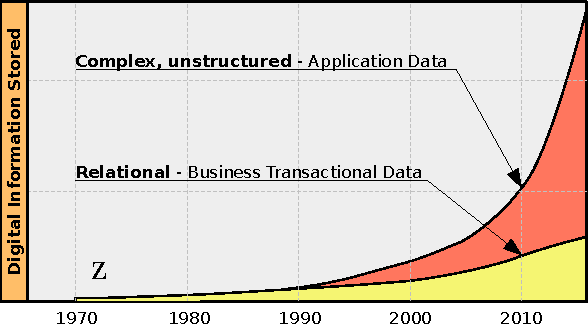
\includegraphics[width=0.99\textwidth]{imagenes/001.pdf}
 \caption{Demand in exponential growth. Source: \emph{Cloudera Inc.}}
\label{fig:datagraph}
\end{center}
\end{figure}

\noindent Over the last years there has been a continuous increase in the quantity of information generated with the Internet as the main driver. Furthermore, this information has reshaped from structured --- and thus, susceptible to being expressed following a relational schema --- to heterogeneous, which has kick-started the necessity to alter the way it is stored and transformed. As the figure \ref{fig:datagraph} shows, those that were the undisputed back-end queens --- relational database systems mostly --- are seeing how their role is fading away due to their incapability to efficiently save unrelated heterogeneity.

As another related dimension, in the year 2000 many .com companies started upgrading their data centers to accommodate the inexorable demand peak that was going to follow. But it never came; and the bubble burst. What happened then was general underutilization --- only \texttt{10\%} of Amazon's global computational resources were in use --- that pushed the search for alternative means to export the surplus as a product. Amazon's own initiative unfolded in 2006 with the \emph{AWS} (\emph{Amazon Web Services}) appearance. AWS, among others, implements a public API for flexible on-demand infrastructure provisioning.

Since then, similar projects have proliferated generalizing how private clusters' unused computational capacity is to be serviced, trying to stay API-compatible with the AWS to facilitate interoperability and thus avoid client's swapping to more flexible providers.

Meanwhile, Google was also in the search for new mechanisms to exploit, with high performance and securely, their own private infrastructure to evolve the capability of their services. MapReduce, as a way to massively execute thousands transformations on input data, became a reality to thrust the generation of Google's humongous inverted index of the Internet \cite{googlemapreduce}. Forthcoming contributions from Nutch's developers --- by that time an Internet search engine prototype --- to the MapReduce paradigm at \emph{Yahoo!}, would traduce into the appearance of today's \emph{de facto} standard in the field: Hadoop. Nowadays Hadoop is used in a myriad of backgrounds, ranging from travel booking sites to storing and servicing mobile data, ecommerce, image processing applications or searching for new forms of energy.

So, by stacking a MapReduce implementation atop elastic infrastructure an optimal exploitation of computational resources would be attainable, rapidly expanding or shrinking them on-demand, while simultaneously reducing the overall energy consumption required to accomplish processings (Figure \ref{fig:energysavings}).

\begin{figure}[tbp]
\begin{center}
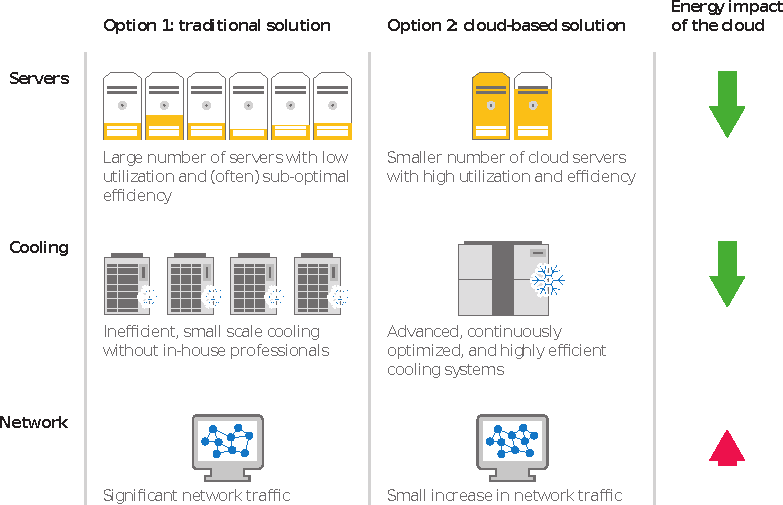
\includegraphics[width=0.99\textwidth]{imagenes/002.pdf}
 \caption{Motivaci\'on energ\'etica. Fuente: \cite{googleapps}}
\label{fig:energysavings}
\end{center}
\end{figure}



\section{Goals}\label{sec:objetivos}

\noindent El objetivo principal de este proyecto es estudiar la posibilidad de desarrollar una soluci\'on que permita dirigir el funcionamiento de un cloud para ejecutar algoritmia codificada siguiendo el paradigma MapReduce, reduciendo al m\'aximo la necesidad de conocimiento de la estructura del cloud concreto utilizado y de los par\'ametros de configuraci\'on de MapReduce.\newline

Para lograrlo se har\'a un an\'alisis pormenorizado de las variadas soluciones de creaci\'on de clouds. Se evaluar\'an sus capacidades y se configurar\'a un entorno de prueba utilizando virtualizaci\'on, que permita extraer conclusiones dirigidas a la elecci\'on de un \emph{framework} en concreto. Una vez completada la primera selecci\'on, se pasar\'a a la evaluaci\'on de los frameworks que soporten las caracter\'isticas del paradigma de programaci\'on MapReduce.\newline

Asimismo, se desarrollar\'a un mecanismo para el env\'io de peticiones de ejecuci\'on de trabajos MapReduce, centr\'andonos en la simplicidad y la universalidad de acceso de la interfaz con el cloud y MapReduce. Sin embargo, la sencillez no ha de representar un obst\'aculo para la explotaci\'on y la obtenci\'on de resultados. Del mismo modo, tanto la seguridad como la privacidad en las comunicaciones y el almacenamiento habr\'an de ser convenientemente definidas; no olvidemos que se trata la construcci\'on de un modelo reducido, a escala, de una soluci\'on que pueda ser implantable en una infraestructura infinitamente m\'as capaz.


\section{Organizaci\'on de la memoria}\label{sec:organizacion}
\noindent El contenido del presente documento se distribuye como se expone a continuaci\'on. Este primer cap\'itulo introduce la l\'inea general de desarrollo del proyecto. El cap\'itulo \ref{cap:estadodelarte} acerca al lector conceptos fundamentales de la \emph{computaci\'on cloud} ---como su arquitectura o la virtualizaci\'on--- y del paradigma MapReduce. El cap\'itulo \ref{cap:evaliaas} describe una evaluaci\'on pr\'actica de cuatro sistemas de manejo de clouds \emph{IaaS}. El cap\'itulo \ref{cap:openstack} explora la estructura modular y el funcionamiento particular de OpenStack Folsom. De forma an\'aloga, el cap\'itulo \ref{cap:hadoop} desvela las peculiarias de Hadoop como framework MapReduce. \newline

Los cap\'itulos subsiguientes se centran en detallar el proyecto desde distintos puntos de vista. El cap\'itulo \ref{cap:solucion} contiene las decisiones de dise\~no y los diagramas UML. El cap\'itulo \ref{cap:rendimiento} recoge los an\'alisis de rendimiento de la soluci\'on en un entorno real de pruebas. El cap\'itulo \ref{cap:conclusiones} analiza trabajos de investigaci\'on experimental relacionados con el proyecto, destacando comparativamente sus caracter\'isticas.  Finalmente, se resumen las principales aportaciones del proyecto y se proponen futuras mejoras a su implementaci\'on. \newline

Adicionalmente se han incluido dos anexos. El ap\'endice \ref{cap:guiainstalacion} recoge una gu\'ia r\'apida para la puesta en funcionamiento de una instalaci\'on del proyecto en un nodo. El ap\'endice \ref{cap:glosario} recoge las explicaciones de ciertos t\'erminos y tecnolog\'ias repartidas por todo el texto.

\cleardoublepage
%\chapter{Background}\label{cap:estadodelarte}
\noindent This second chapter tries to acquaint the reader with the key concepts that define Cloud Computing as well as the MapReduce archetype. Later chapters will elaborate on top of them.

\section{Cloud Computing}\label{sec:computacioncloud}
\noindent As it has already been discussed, Cloud Computing is, in essence, a distributed computing model that attempts to ease the on-demand consumption of computational infrastructure, by exporting it as virtual computational resources, platforms or services. However it may seem, Cloud Computing is no new technology; it introduces a new way to exploit idle computing capacity. What it intends is to make orchestration of enormous data centers more flexible, so as to let a user start or destroy virtual machines as required --- Infrastructure as a Service (\emph{IaaS}) ---, leverage a testing environment over a particular operating system or software platform --- Platform as a Service (\emph{PaaS}) --- or use a specific service like remote backup --- Software as a Service (\emph{SaaS}). Figure \ref{fig:cloudlayers} shows the corresponding high level layer diagram of a generic cloud.

\begin{figure}[tbp]
\begin{center}
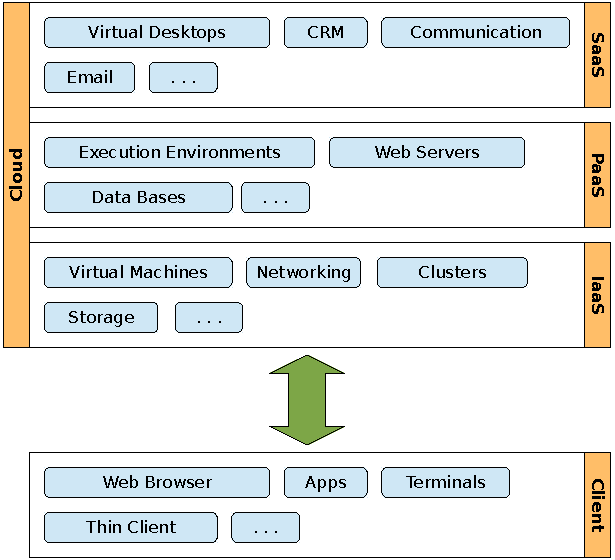
\includegraphics[width=0.69\textwidth]{imagenes/003.pdf}
 \caption{Software layers in a particular cloud deployment}
\label{fig:cloudlayers}
\end{center}
\end{figure}

Different IaaS Frameworks will cover the functionality that is required to drive the cloud-defining \emph{physical} infrastructure. Nonetheless, an effort to analyze, design, configure, install and maintain the intended service will be needed, bearing in mind that the degree of elaboration grows from IaaS services to SaaS ones. In effect, PaaS and SaaS layers are stacked supported by those immediately under --- as happens with software in general which is implemented over a particular platform which, in turn, is also build upon a physical layer. Every Cloud Framework focuses on giving the option to configure a stable environment in which to run virtual machines whose computing capabilities are defined by four variables: Virtual CPU count, virtual RAM, virtual persistent memory and virtual networking devices. Such an environment makes it possible to deploy virtual clusters upon which to install platforms or services to be subsequently consumed by users, building up the software layers that conform PaaS and SaaS paradigms respectively.

No less important features like access control, execution permissions, quota or persistent or safe storage will also be present in every framework.

\subsection{Architecture}\label{subsec:arquitecturacloud}
\noindent Figure \ref{fig:cloudlayers} showed possible layers that could be found in a cloud deployment. Depending on the implemented layers, the particular framework and the role played by the cluster node different particular modules will appear, making it possible to consume the configured services. These modules may be though of as cloud subsystems that connect each one of the parts that are required to execute virtual machines. Those virtual machines' capabilities are defined by the four variables previously discussed --- VCPUS, RAM, HDD and networking. As there is no methodology guiding how those subsystems should be in terms of size and responsibility, each framework makes its own modular partition regarding infrastructure management.

Setting modularity apart, one common feature among different clouds is the separation of responsibility in two main roles: \emph{Cloud Controller} and \emph{Cloud Node}. Figure \ref{fig:archcloud} shows a generic cloud deployment in a cluster with both roles defined. The guidelines followed for having this two roles lay close to the \emph{Master-Slave} architecture approach. In those, in general, there's a set of computers labeled as coordinators which are expected to control execution, and another set made up with those machines that are to carry out the actual processing.

\begin{figure}[tbp]
\begin{center}
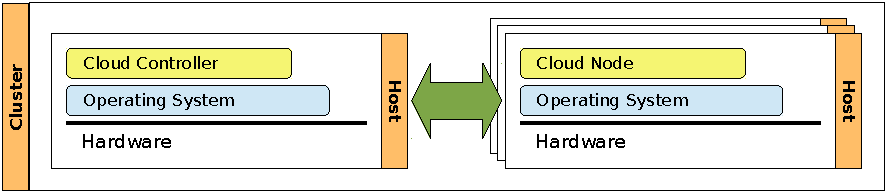
\includegraphics[width=0.9\textwidth]{imagenes/004.pdf}
 \caption{Cloud Controller and Cloud Node}
\label{fig:archcloud}
\end{center}
\end{figure}

In a cluster, host computers or cluster nodes --- labeled as Cloud Controllers or Cloud Nodes --- cooperate in a time synchronized fashion with \emph{NTP} (\emph{Network Time Protocol}) and communicate via message passing supported by asynchronous queues. To store services' metadata and status they typically draw upon a \emph{DBMS} (\emph{Data Base Management System}) implementation, which is regularly kept running in a dedicated cluster node, or sharded (distributed) among the members of the database federation.

Although there is no practical restriction to configuring both Cloud Controller and Cloud Node within a single machine in a cluster, this approach should be limited to development or prototyping environments due to the considerable impact in performance that it would imply.

\subsubsection{Cloud Controller}\label{subsubsec:cloudcontroller}
\noindent The fundamental task of a Cloud Controller is to maintain all of the cloud's constituent modules working together by coordinating their cooperation. As an example, it is a Controller's duty to:

\begin{itemize}
 \item Control authentication and authorization.
 \item Recount available infrastructure resources.
 \item Manage quota.
 \item Keep track of usage balance.
 \item Maintain an inventory of users and projects.
 \item Expose an API for service consumption.
 \item Monitor the cloud in real time.
\end{itemize}

Being an essential part of a cloud as it is, the Controller node is usually replicated in physically distinct computers. Figure \ref{fig:cloudcontroller} shows a Cloud Controller's architecture from a high level perspective.

\begin{figure}[tbp]
\begin{center}
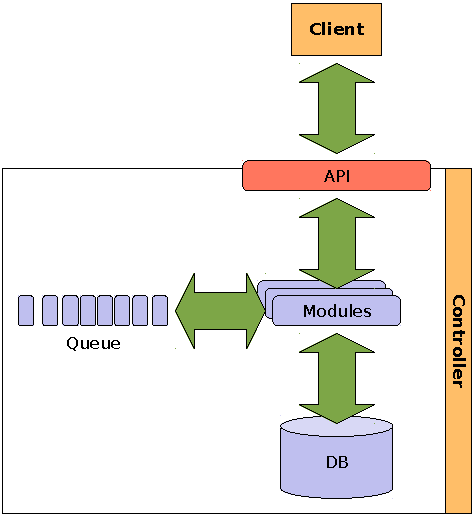
\includegraphics[width=0.5\textwidth]{imagenes/005.pdf}
 \caption{Cloud Controller in detail}
\label{fig:cloudcontroller}
\end{center}
\end{figure}

As a general rule, clients will interact with the cloud through a Web Service API --- \emph{RESTful} APIs (\emph{REpresentational State Transfer}) mostly. Those APIs vary slightly from company to company, as usual, which forces clients to be partially coupled to the cloud implementation they intend to use. That is why there has been an increasing trend for unifying and standardizing those APIs in order to guarantee compatibility inter-framework. Of special mention is the cloud standard proposed by the \emph{Open Grid Forum}: \emph{OCCI} (\emph{Open Cloud Computing Interface} \cite{occisdraft}).

Cloud's modules support its functional needs. Each one of them will have a well-defined responsibility, and so, there will appear networking-centered modules, access and security control modules, storage modules, etc. Many of them existed before the advent of Cloud Computing, but they worked only locally to a cluster or organization. Inter-module communication is handled by an asynchronous message queue that guarantees an efficient broadcasting system outside of the Cloud Controller --- the rest of the cluster nodes participating in the cloud.

To store and expose configuration data to the cluster in a single place while managing concurrent requests to update these data, every IaaS Framework evaluated resorts to a DBMS.

Hardware requirements on the cluster nodes vary from each particular framework implementation and the \emph{QoS} expected, but, they generally require something around 10 GB of RAM, quad core CPU, Gigabit Ethernet and one TB of storage to get started.


\subsubsection{Cloud Node}\label{subsubsec:cloudnode}
\noindent If the Cloud Controller is entrusted the cloud's correct functioning acting like glue for its parts, the actual task processing is performed in the Cloud Nodes using the VCPU, VRAM, VHDD that are going to be borrowed from the corresponding CPU, RAM and HDD from the real nodes of the cluster.

Cloud Nodes may be heterogeneous according to their hardware characteristics. They will configure a resource set that, seen from outside of the cluster, will appear to be a homogeneous whole where the summation of capacities of every participating node is the cloud's dimension. Furthermore, this homogeneous space could be provisioned, as discussed, on-demand. It is the Cloud Controller's responsibility to single out the optimal distribution of virtual servers throughout the cluster, attending to the physical aspects of both the virtual machine and the computer in which it will run.

The most important subsystem in a Cloud Controller is the \emph{hypervisor} or \emph{VMM} (\emph{Virtual Machine Monitor}). The hypervisor is responsible for making possible the execution of virtual servers --- or virtual instances --- by creating the virtual architecture needed and the \emph{virtual execution domain} that will be managed with the help of the kernel of the operating system. To generate this architecture there fundamentally exist three techniques: \emph{Emulation}, \emph{Paravirtualization} and \emph{Hardware Virtualization} --- or \emph{Full Virtualization}. Different hypervisors support them in different degree, and most will only cover one of them.

\subsection{Virtualization Techniques}\label{subsec:tecnicasemu}
\noindent What follows is a brief review of the main methods to create virtual infrastructure.

\subsubsection{Emulation}\label{subsubsec:emulacion}
\noindent Emulation is the most general virtualization method, in a sense that it does not call for anything special be present in the underlying hardware. However, it also carries the highest penalization in terms of performance. With emulation, every structure sustaining the virtual machine operation is created as a functional software copy of its hardware counterpart; i.e., every machine instruction to be executed in the virtual hardware must be run software-wise first, and then be translated on the fly into another machine instruction runnable in the physical domain --- the cluster node. The interpreter implementation and the divergence between emulated and real hardware will directly impact the translation overhead. This fact hinders the emulation from being widely employed in performance-critical deployments. Nonetheless, thanks to its operating flexibility, it's generally used as a mechanism to support legacy systems or as a development platform. Besides, the kernel in the guest operating system --- the kernel of the virtual machine operating system --- needs no alteration whatsoever, and the cluster node kernel need only load a module.

\subsubsection{Hardware Virtualization}\label{subsubsec:virthardware}
\noindent Hardware Virtualization, on the contrary, allows host's processes to run directly atop the physical hardware layer with no interpretation. Logically, this provides a considerable speedup from emulation, though it imposes a special treatment to be given to virtual processes. Regarding CPUs, both AMD's and Intel's support virtual process execution --- which is the capacity to run processes belonging to the virtual domain with little performance overhead --- as far as convenient hardware extensions are present (\emph{SVM} and \emph{VT-x} respectively \cite{intelvtx}). Just as happened with emulation, an unaltered host kernel may be used. This fact is of relative importance as if wasn't so it would limit the myriad of OSs that could be run as guests. Lastly, it should be pointed out that the hardware architecture is exposed to the VM as it is, i.e. with no software middleware or transformation.

\subsubsection{Paravirtualization}\label{subsubsec:paravirt}
\noindent Paravirtualization uses a different approach. To begin with, it is indispensable that the guest kernel be modified to make it capable of interacting with a paravirtualized environment. When the guest runs, the hypervisor will separate the regions of instructions that have to be executed in kernel mode in the CPU, from those in user mode which will be executed as regular host instructions. Subsequently, the hypervisor will manage an on-contract execution between host and guest allowing the latter to run kernel mode sections as if they belonged to the real execution domain --- as if they were instructions running in the host, not in the guest --- with almost no performance penalty. Paravirtualization, in turn, does not require an special hardware extension be present in the CPU.

\subsection{Cloud IaaS frameworks}\label{subsec:frameworksiaas}
\noindent Cloud IaaS Frameworks are those software systems managing the abstraction of complexity associated with on-demand provisioning and administering failure-prone generic infrastructure. In spite of being almost all of them open-sourced --- which fosters reusability and collaboration ---, they have evolved in different contexts. This fact has raised the condition of lacking interoperability among them, maturing non-standard APIs; though today those divergences are fading away. These frameworks and APIs are product of the efforts to improve and ease the control of the underlying particular clusters of machines on which they germinated. Thus, it is no surprising their advances had originated in parallel with the infrastructure they drove, leaving compatibility as a secondary issue.

Slowly but steadily these managing systems became larger in reach and responsibility boosted by an increasing interest in the sector. It happened that software and systems engineering evolved them into more abstract software packages capable of managing more different physical architectures. AWS appearance finished forging the latent standardization need, and as of today, most frameworks try to define APIs close to Amazon's --- nowadays the de-facto standard --- and OCCI's \cite{occisdraft}.

\section{MapReduce Paradigm}\label{sec:mapred}
\noindent The origin of the paradigm centers around a publication by two Google employees \cite{googlemapreduce}. In this paper they explained a method implementation devised to abstract the common parts present in distributed computing that rendered simple but large problems much more complex to solve when paralleling their own code on massive clusters.

A concise definition states that MapReduce is ``\emph{a data processing model and execution environment that runs on large clusters of commodity computers}'' \cite{hadoopdefguide}.

\subsection{Programming Model}\label{subsec:programacionmapred}
\noindent The MapReduce programming model requires the developer express problems as a partition of two well-defined pieces. A first part deals with the reading of input data and with producing a set of intermediate results that will be scattered over the cluster nodes. These intermediate transformations will be grouped according to an intermediate key value. A second phase begins with that grouping of intermediate results, and concludes when every \emph{reduce} operation on the groupings succeeds. Seen from another vantage point, the first phase corresponds, broadly speaking, to the behavior of the functional \emph{map} and the second to the functional \emph{fold}.

In terms of the MapReduce model, these functional paradigm concepts have given rise to \emph{Map} and \emph{Reduce} functions. Both Map and Reduce have to be supplied by the developer, which may require a deviation in the thinking process of the developer in breaking down the original problem towards a coded solution. As counterpart, the MapReduce model will deal with parallelizing the computation, distributing input data across the cluster, handling exceptions that could raise during execution and recovering output results; everything transparent to the engineer.

\subsubsection{Map Function}\label{map}
\noindent The typical functional map takes any function \emph{F} and a list of elements \emph{L} or, in general, any recursive data structure, to return a list resulting from applying \emph{F} to each element of \emph{L}. Figure \ref{fig:functionalmap} shows its signature and an example.

\begin{figure}[tbp]
\begin{center}
\begin{tabular}{|l|}
\hline
$\mathbf{map:} \: \left ( \alpha \rightarrow \beta \right ) \: \rightarrow \: \alpha \: list \: \rightarrow \: \beta \: list$ \\
$\mathbf{map} \: \left( \mathbf{pow}\:2 \right) \: \left[ 1,2,3 \right] \: \Rightarrow \: \left[ 1,4,9 \right ]$ \\
\hline
\end{tabular}
\caption{Map function example (functional version)}
\label{fig:functionalmap}
\end{center}
\end{figure}

In its MapReduce realization, the map function receives a tuple as input and produces another tuple \emph{(key, value)} as intermediate output. It is the MapReduce library's responsibility to feed the map function by transforming the data contained in input files into \emph{(key, value)} pairs. Then, after the mapping has been completed, it deals with grouping those intermediate tuples by key before passing them in as input to the reduce function. Input and output data types correspond to those shown in the function signature figure \ref{fig:mapreducemap}.

\begin{figure}[tbp]
\begin{center}
\begin{tabular}{|l|}
\hline
$\mathbf{map:} \: \left( k1,v1 \right) \: \rightarrow \: \left( k2,v2 \right) list$ \\
$\mathbf{k:} \: clave \linebreak$ \\
$\mathbf{v:} \: valor \linebreak$ \\
$\mathbf{\left(kn,vn \right):} \: par \: \left( clave,valor \right) \: en \: un \: dominio \: n$ \\
\hline
\end{tabular}
\caption{Map function signature (MapReduce version)}
\label{fig:mapreducemap}
\end{center}
\end{figure}


\subsubsection{Reduce function}\label{reduce}
\noindent The typical functional fold expects any function \emph{G}, a list \emph{L}, or generally any type of recursive data type, and any initial element \emph{I}, subtype of \emph{L}'s elements. Fold returns the value in \emph{I} resulting from building up the intermediate values generated after applying \emph{G} to each element in \emph{L}. Figure \ref{fig:fold} presents fold's signature as well as an example.

\begin{figure}[tbp]
\begin{center}
\begin{tabular}{|l|}
\hline
$\mathbf{fold:} \: \left( \alpha \rightarrow \beta \rightarrow \alpha \right) \: \rightarrow \: \alpha \: \rightarrow \: \beta \: list \: \rightarrow \: \alpha$ \\
$\mathbf{fold} \: \left( \mathbf{+} \right) \: 0 \: \left[ 1,2,3 \right] \: \Rightarrow \: 6$ \\
\hline
\end{tabular}
\caption{Fold function example}
\label{fig:fold}
\end{center}
\end{figure}

Contrary to map, reduce expects the intermediate groups as input to produce a smaller set of values for each group as output, because reduce will iteratively \emph{fold} the groupings into values. Those reduced intermediate values will be passed in again to the reduce function if more values with the same key appeared as input. Reduce's signature is shown on figure \ref{fig:reduce}. Just as happens with map, MapReduce handles the transmission of intermediate results out from map into reduce. The model also describes the possibility to define a \emph{Combiner} function that would act after map partially reducing the values with the same key to lower network traffic --- the combiner usually runs in the same machine as the map.

\begin{figure}[tbp]
\begin{center}
\begin{tabular}{|l|}
\hline
$\mathbf{reduce:} \: \left( k2,v2 \: list \right) \: \rightarrow \: v2 \: list$ \\
$\mathbf{k:} \: clave$ \\
$\mathbf{v:} \: valor$ \\
$\mathbf{\left(kn,vn \right):} \: par \: \left(clave,valor\right) \: en \: un \: dominio \: n$ \\
\hline
\end{tabular}
\caption{Reduce function signature}
\label{fig:reduce}
\end{center}
\end{figure}

\subsubsection{A word counter in MapReduce}\label{subsubsec:wordcount}
\noindent As an example, figure \ref{fig:wordcount} shows the pseudocode of a MapReduce application to count the number of words in a document set.

\begin{figure}[tbp]
 \begin{center}
  \begin{tabular}{|l|}
   \hline
   \texttt{{\bf Map} (String key, String value):} \\
   \texttt{// key: document name} \\
   \texttt{// value: document contents} \\
   \texttt{{\bf for each} word w {\bf in} value:} \\
   \texttt{{\bf EmitIntermediate} (w, ``1'')};\\ \\

   \texttt{{\bf Reduce} (String key, Iterator values):} \\
   \texttt{// key: a word} \\
   \texttt{// values: an Iterable over intermediate counts of the word key} \\
   \texttt{{\bf int} result = 0;} \\
   \texttt{{\bf for each} v {\bf in} values:} \\
   \texttt{{\bf Emit} ({\bf AsString} (result));} \\
   \hline
  \end{tabular}
  \caption{MapReduce wordcount pseudocode. Source: \cite{googlemapreduce}}
  \label{fig:wordcount}
 \end{center}
\end{figure}

In a Wordcount execution flow the following is going to happen: map is going to be presented a set of names containing all of the documents in plain text whose words will be counted. Map will subsequently iterate over each document in the set emitting the tuple \emph{(<word>, ``1'')} for each word found. Thus, an explosion of intermediate pairs will be generated as output of map, which will be distributed over the network and progressively folded in the reduce phase. Reduce is going to be input every pair generated by map but under a different form. Reduce will accept on each invocation the pair \emph{(<word>, list(``1''))}. The list of \emph{``1''}s, or generically, an \texttt{Iterable} over \emph{``1''}s, will contain as many elements as instances of the word \emph{<word>} there were in the document set --- this supposing the map phase were over before starting the reduce phase and that every word \emph{<word>} were submitted to the same reducer in the cluster --- a cluster node executing the reduce function.

Once the flow had been completed, MapReduce would return a listing with every word in the documents and the number of times it appeared.

\subsection{Applicability of the Model}\label{subsec:aplicabilidad}
\noindent The myriad of problems that could be expressed following the MapReduce programming paradigm is clearly reflected in \cite{googlemapreduce}, a subset of them being:

\begin{itemize}
 \item Distributed grep: Map emits every line matching the regular expression. Reduce only forwards its input to its output acting as the identity function.
 \item Count of URL access frequency: Like wordcount, but with the different URLs as input to map.
 \item Reverse web-link graph: For each URL contained in a web document, map generates the pair \emph{(<target\_URL>, <source\_URL>)}. Reduce will emit the pair \emph{(target, list(source))}.
 \item Inverted index: Map parses each document and emits a series of tuples in the form \emph{(<word>, <document\_id>)}. All of them are passed as input to reduce that will generate the sequence of pairs \emph{(<word>, list(document\_id))}.
\end{itemize}

\subsection{Processing Model}\label{subsec:processingmodel}
\noindent Besides defining the structure that the applications willing to leverage MapReduce capabilities will have to follow --- so that they need not code their own distribution mechanisms ---, with \cite{googlemapreduce} an implementation of the model was introduced which allowed Google to stay protocol, architecture and system agnostic while keeping their commodity clusters on full utilization. This agnosticism allows for deploying vendor-lock free distributed systems.

The MapReduce model works by receiving self-contained processing requests called \emph{job}s. Each job is a \emph{partition} of smaller duties called \emph{task}s. A job won't be completed until no task is pending for finishing execution. The processing model main intent is to distribute the tasks throughout the cluster in a way that reduced job latency. In general, task processing on each phase is done in parallel and phases execute in sequence; yet, it is not technically needed for reduce to wait until map is complete.

Figure \ref{fig:exmapreduce} shows a summary of a typical execution flow. It is interesting enough to deepen in its details as many other MapReduce implementations will present similar approaches.

\begin{figure}[tbp]
\begin{center}
 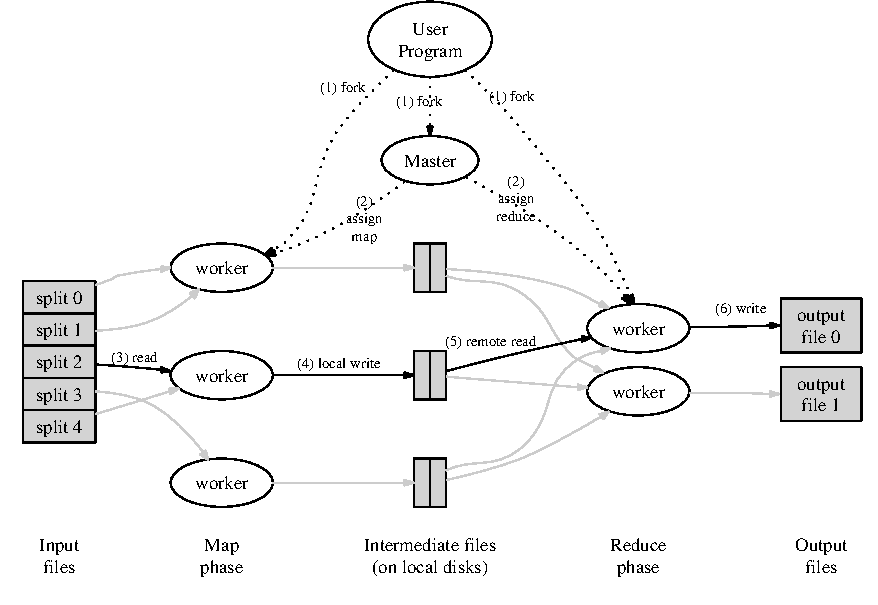
\includegraphics[width=0.9\textwidth]{imagenes/006.pdf}
 \caption{MapReduce execution diagram. Source: \cite{googlemapreduce}}
 \label{fig:exmapreduce}
\end{center}
\end{figure}

\begin{enumerate}
 \item MapReduce divides input files in \emph{M} parts, the size of which is controlled with a parameter, and distributes as many copies of the MapReduce user algorithm as nodes participate in the computation.
 \item From this moment onward, each program copy resides in a cluster node. A random copy is chosen among them and is labeled as the \emph{Master Replica}, effectively assigning the \emph{Master Role} to the node holding the replica; every other node in the cluster is designated with the \emph{Worker Role}. Those worker nodes will receive the actual MapReduce tasks and their execution will be driven by the master node. There will be \emph{M} map tasks and \emph{R} reduce tasks.
 \item Workers assigned map tasks read their corresponding portions of the input files and parse the contents generating tuples \emph{(key, value)} that will be submitted to the map function for processing. Map outputs are stored in memory as cache.
 \item Periodically, those pairs in memory are \emph{spilt} to a local disk and partitioned into \emph{R} regions. Their path on disk is then sent back to the master, responsible for forwarding these paths to \emph{reduce workers}.
 \item Now, when a reducer is notified that it should start processing, the path to the data to be reduced is send along and the reducer will fetch it directly from the mapper via \emph{RPC} (\emph{Remote Procedure Call}). Before actually invoking the reduce function, the node itself will sort the intermediate pairs by key.
 \item Lastly, the reducer iterates over the key-sorted pairs submitting to the user-defined reduce function the key and the \texttt{Iterable} of values associated with the key. The output of the reduce function is appended to a file stored over the distributed file system.
\end{enumerate}

When every map and reduce tasks had succeeded, the partitioned output space --- the file set within each partition --- would be returned back to the client application that had made the MapReduce invocation.

This processing model is abstract enough as to be employed to the resolution of very large problems running on huge clusters.

\subsection{Fault Tolerance}\label{subsec:toleranciafallos}
\noindent The idea of providing an environment to execute jobs long enough to require large sets of computing machines to keep the latency within reasonable timings, calls for the definition of a policy able to assure a degree of tolerance to failure. If unattended, those failures would lead to errors; some would cause finished tasks to get lost, others would put intermediate data offline. Consequently, if no measures were taken to prevent or deal with failure, job throughput would humble as some would have to be rescheduled all along.

The MapReduce model describes a policy foreseeing a series of issues within an execution flow, and duly implements a series of actions to prevent them.

\subsubsection{Worker Failure}\label{subsubsec:fallotrabajador}
\noindent The least taxing of the problems. To control that every worker is up, the master node polls them periodically. If a worker did not reply to pings repeatedly, it would be marked as failed.

A worker marked failed will neither be scheduled new tasks nor will be remotely accessed by reducers to load intermediate map results that it may had; a fact that could prevent the workflow from succeeding. If so were the case, the access to these data would be resolved by the master labeling the results of the failing tasks as \emph{idle}, so that they could be rescheduled at a later time to store the results in an active worker.

\subsubsection{Master Failure}\label{subsubsec:fallomaestro}
Failure of a master node is more troublesome. The proposed approach consists in making the master periodically create a snapshot from which to restore to a previous state if it went unexpectedly down. It is a harder problem than a worker failure mainly because there can only be one master per cluster, and the time it would take another node to take over the master role would leave the scheduling pipeline stalled. The master being in a single machine has, nonetheless, the benefit of lowering the probability of failure --- this is precisely why the Google MapReduce paper \cite{googlemapreduce} had put forward that the entire job be canceled. Still, as it is no good design decision to leave a \emph{single point of failure}, subsequent MapReduce implementations have proposed to replicate the master in other nodes in the same cluster.

\subsection{Aditional Characteristics}\label{subsec:caracteristicasadicionales}
\noindent What follows is a summary of additional features of the original MapReduce implementation.

\subsubsection{Locality}\label{subsubsec:localidad}

\noindent The typical bottleneck in modern distributed deployments is network bandwidth. In MapReduce executions, the information flows into the cluster from an external client. As already discussed, each node in a MapReduce cluster holds a certain amount of the input data and shares its processing capacity to be used for particular MapReduce tasks over those data. Each stage in the MapReduce executing pipeline requires a lot of traffic to be handled by the network which would reduce throughput if no channel wide enough were deployed nor a locality exploiting strategy were implemented.

In fact, MapReduce explores a method to use locality as an additional resource. The idea is for the distributed file system to place data as close as possible to where they will transformed --- it will try to store map and reduce data close to the mappers and reducers that will transform those data ---, effectively diminishing the transport over the network.

\subsubsection{Complexity}\label{subsubsec:complejidad}
\noindent A priori, variables \emph{M} and \emph{R}, the number of partitions of the input space and of the intermediate space respectively, may be configured to take any value whatsoever. Yet, there exist certain practical limits to their values. For every running job the master will have to make $O(M + R)$ scheduling decisions --- if no error forced the master to reschedule tasks ---, as each partition of the input space will have to be submitted to a mapper and each intermediate partition will have to be transmitted to a reducer, coming to $O(M + R)$ as the expression of \emph{temporal complexity}. Regarding \emph{spatial complexity}, the master will have to maintain $O(M \cdot R)$ as piece of state in memory as the intermediate results of a map task may be propagated to every piece \emph{R} of the reduce space.

\subsubsection{Backup Tasks}\label{subsubsec:secundarias}
\noindent A situation could arise in which a cluster node be executing map or reduce tasks much slower than it theoretically could. Such a circumstance may arise with a damaged drive which would cause read and write operations to slow down. Since jobs complete when all of its composing tasks had been finished, the faulted node (\emph{the straggler}) would be curbing the global throughput. To alleviate this handicap, when only few tasks are left incomplete for a particular job, \emph{Backup Task}s are created an submitted to additional workers, making a single task be executed twice concurrently. By the time one copy of the task succeeded it would be labeled \emph{completed}, duly reducing the impact of stragglers at the cost of wasting computational resources.

\subsubsection{Combiner Function}\label{subsubsec:combiner}

\noindent Many times it happens that there exists a good number of repeated intermediate pairs. Taking wordcount as an example, it can be easily seen that every mapper will generate as many tuples \emph{(``a'', ``1'')} as \emph{a}'s there are in the input documents. A mechanism to lower the tuples that will have to be emitted to reducers is to allow for the definition of a \emph{Combiner Function} to group outputs from the map function, in the same mapper node, before sending them out over the network, effectively cutting down traffic.

In fact, it is usual for both combiner and reduce functions to share the same implementation, even though the former writes its output to local disk while the latter writes directly to the distributed file system.

\subsection{Other MapReduce Implementations}\label{subsec:frameworksmapred}
\noindent Since 2004 multiple frameworks that implement the ideas exposed in the paper \cite{googlemapreduce} have been coming out. The next listing clearly shows the impact MapReduce has created.

\begin{description}
 \item[Hadoop] \cite{hadoopdefguide} One of the first implementations to cover the MapReduce processing model and framework of reference to other MapReduce codifications. It is by far the most widely deployed, tested, configured and profiled today.
 \item[GridGain] \cite{gridgainvshadoop} Commercial and centered around in-memory processing to speedup execution: lower data access latency at the expense of smaller I/O space.
 \item[Twister] \cite{twister} Developed as a research project in the University of Indiana, tries to separate and abstract the common parts required to run MapReduce workflows in order to keep them longer in the cluster distributed memory. With such an approach, the time taken to configure mappers and reducers in multiple executions is lowered by doing their setup only once. \emph{Twister} really shines in executing \emph{iterative} MapRecude jobs --- those jobs where maps and reduces do not finish in sequence and only once, but need instead a multitude of complete map-reduce cycles to complete.
 \item[GATK] \cite{gatk} Used for genetic research to sequence and evaluate DNA fragments from multiple species.
 \item[Qizmt] \cite{qizmt} Written in C\# and deployed for MySpace.
 \item[misco] \cite{misco} Written 100\% Python and based on previous work at Nokia, it is posed as a MapReduce implementation capable of running in mobile devices.
 \item[Peregrine] \cite{peregrine} By optimizing how intermediate results are transformed and by passing every I/O operation through an asynchronous queue, its developers claim to have formidably accelerated task execution rate.
 \item[Mars] \cite{mars} Implemented in \emph{NVIDIA CUDA}, it revolves around extracting higher performance by moving the map and reduce operations into the graphics card. It is supposed to improve processing throughput by over an order of magnitude.
\end{description}

Hadoop is undoubtedly the most used MapReduce implementation nowadays. Its open-source nature and its flexibility, both for processing and storage, have been reporting back an increasing interest from the IT industry. This has brought out many pluggable extensions that enhance Hadoop's applicability and usage.

%\cleardoublepage
%\chapter{Experimental Assessment of IaaS Clouds}\label{cap:evaliaas}

\noindent In this chapter we will be reviewing the most used frameworks to drive IaaS Clouds. An initial selection will be made and it will be progressively shrunk following certain criteria like maturity, ease of use or documentation quality, until one remains. A deep study will be carried out on that prevailing one.

\section{Metodolog\'ia de evaluaci\'on}\label{sec:evaluacion}

\noindent A thorough evaluation of the capabilities of the different frameworks is not possible unless an actual deployment is carried through. The virtual infrastructure that is generated when a cloud has finished installing, no matter how small the deployment, is large and complex. Besides, trying to \emph{emulate} the real hardware that will support the cloud is meager at times, e.g. if full hardware virtualization were used, the hypervisor would have to be allowed direct access to the CPU. \emph{Nested Hardware Virtualization} --- the capacity for a CPU to export its native virtualization capabilities to a guest running atop a host node, or the ability to use full hardware virtualization \emph{inside} a virtual machine ---, does not currently enjoy widespread adoption as it requires implementation efforts from both CPU designers and virtualization software developers. This means that it will not be possible for us to appraise the myriad IaaS Cloud solutions by creating a virtual cluster over which to deploy our clouds. Nonetheless, it will be the first test that the frameworks will have to pass in order to be eligible for further assessment, as it is clear reflection of their virtualizing flexibility.

To diagnose the superiority of one of them over the rest, a scaled down setup will be completed to evaluate the proficiency in maintaining the IaaS service running in spite of the reduced infrastructure. Quality and transparency in the documentation, as well as community support and engagement will also be born in mind.

The testing environment follows the organization shown in figure \ref{fig:espacioprueba}.

\begin{figure}[tbp]
\begin{center}
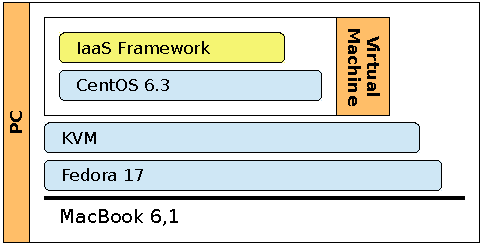
\includegraphics[width=0.55\textwidth]{imagenes/007.pdf}
 \caption{General testing space}
\label{fig:espacioprueba}
\end{center}
\end{figure}

\section{Evaluated Frameworks}\label{sec:frameworksevaluados}

\noindent The frameworks are:
\begin{itemize}
 \item CloudStack %3.0.2
 \item Eucalyptus %3.1.1
 \item OpenNebula %3.8.1
 \item OpenStack
\end{itemize}

From an exclusively functional vantage point, the four of them cover clearly the requirements imposed with the project, which, in short, it would be the faculty to run and manage the lifecycle of an indeterminate number of custom VMs, tailored for MapReduce executions, through an API that would allow for the definition of a simple job control interface.

\emph{Eucalyptus} and \emph{OpenStack} take a more modular approach to the solution, unveiling smaller functional parts, while at the same time decoupling those modules. With a module set in this fashion, installations become more flexible and tougher on par. However, to contain the operative effort, OpenStack ships with a series of scripts that help managing its deployments. Regarding their system requirements, they all support installations in modern Linux distributions with KVM or Xen as hypervisors. When dealing with a real deployment, the framework of choice will likely depend more on the existing platform than on particular limitations that any cloud may have.

As a side note, it is remarkable the lack of interoperability among them. All of them try to adhere to the AWS API in different degree --- some of them partially support it, others use \emph{adaptors} to it. OpenNebula, OpenStack and Eucalyptus have demonstrated to be carrying on coding efforts to fully support the OGF's standard: OCCI.

%\subsection{Eucalyptus}\label{subsec:eucaliptus}

Eucalyptus, in spite of being the first to fully cover the AWS API, which is merely anecdotic nowadays, shows two obstacles that hinder its evaluation. First, it is not fully open sourced:\texttt{VMware Broker} which brings the opportunity to use virtualized infrastructure based on  VMware technology, is only available to paid subscribers. And second, it is impossible to setup Eucalyptus within a VM to test start-up time or installation complexity, for example, as it explains its installation guide \cite{eucainstall}. Both obstacles make Eucalyptus back out from the evaluation list. The rest have been compared after their setting up and configuration.

\subsection{CloudStack}\label{subsec:cloudstack}

\noindent En \cite{cloudstackquickinstall} se describe la instalaci\'on r\'apida de la \'ultima versi\'on de CloudStack bajo la tutela exclusiva de Citrix. Claramente determina que los nodos de cloud tienen que soportar, como para Eucalyptus, extensiones de vir\-tua\-li\-za\-ci\'on hardware (VT-x o AMD-V) para poder arrancar m\'aquinas virtuales sobre \emph{XenServer} o KVM. Sin embargo, la importancia de que CloudStack pasar\'ia a formar parte de \emph{The Apache Software Foundation} a partir de la versi\'on 4 como proyecto en incubaci\'on \cite{cloudstackstrategy}, y la realidad de un art\'iculo t\'ecnico de Citrix que abr\'ia la puerta a despliegues sobre anfritriones sin extensiones de virtualizaci\'on hardware \cite{cloudstacknohvm} ---a pesar de que incluso el manual de instalaci\'on de CloudStack 4 \cite{apachecloudstack4} siga contemplando esa limitaci\'on---, hizo que se ajustase el entorno de ejecuci\'on de la figura \ref{fig:cloudstack}.\newline

\begin{figure}[tbp]
\begin{center}
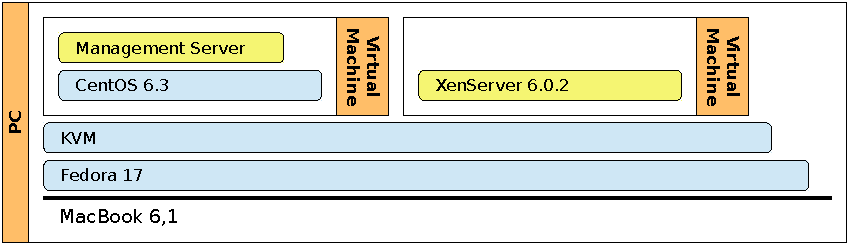
\includegraphics[width=0.99\textwidth]{imagenes/008.pdf}
 \caption{CloudStack 3.0.2 con XenServer como hipervisor}
\label{fig:cloudstack}
\end{center}
\end{figure}

Siguiendo las gu\'ias de instalaci\'on r\'apida y avanzada ---\cite{cloudstackquickinstall} y \cite{cloudstackadvinstall} res\-pec\-ti\-va\-men\-te---, el proceso se puede resumir en los pasos siguientes:

\begin{itemize}
 \item Se crearon dos m�quinas virtuales para contener el \emph{Management Server} (\emph{MS}) de CloudStack y el hipervisor XenServer: 1 GB RAM para el MS, 3 GB RAM para Xen y 20 GB HDD, \emph{ACPI} y \emph{APIC} para ambos.
 \item Para el MS:
  \begin{itemize}
      \item Se descarg\'o, instal\'o y actualiz\'o \emph{CentOS 6.3}.
   \item Se nombr\'o \emph{cloudstack} a la m\'aquina virtual.
   \item Igualmente nombrado, se dio de alta un nuevo usuario, \emph{cloudstack}, y se agreg\'o a la lista de \emph{sudoers}.
   \item Se sigui\'o la gu\'ia de instalaci\'on \cite{cloudstackquickinstall} para concluir el proceso.
  \end{itemize}
 \item Para Xen:
  \begin{itemize}
   \item Se descarg\'o la versi\'on 6.0.2 de XenServer desde la web de Citrix.
   \item Se siguieron los apuntes de la gu\'ia de instalaci\'on de CloudStack \cite{cloudstackquickinstall} y el manual de configuraci\'on de XenServer \cite{xenserverinstall} para realizar la instalaci\'on.
  \end{itemize}
 \item Adicionalmente:
  \begin{itemize}
   \item Antes de crear la zona de ejecuci\'on y definir el cl\'uster, el almacenamiento primario y secundario, etc., se tuvo que modificar la opci\'on de configuraci\'on global para permitir anfitriones sin extensiones de virtualizaci\'on hardware \cite{cloudstacknohvm}.
   \item Una vez verificado el correcto reconocimiento de la infraestructura:
    \begin{itemize}
     \item Se copi\'o la imagen de CentOS 6.3 al MS.
     \item Se arranc\'o un \texttt{SimpleHTTPServer} en el puerto \texttt{443} del MS.
     \item Se permiti\'o el acceso al puerto \texttt{443}, desde \texttt{iptables}, en el MS.
     \item Se carg\'o la imagen en el cloud desde la interfaz web.
    \end{itemize}
  \end{itemize}
\end{itemize}


\subsection{OpenNebula}\label{subsec:opennebula}
\noindent En comparaci\'on con el procedimiento anterior, el esfuerzo de instalaci\'on de OpenNebula 3.8 es muy inferior. De \cite{centosonquickstart} se deriva el proceso que se sigui\'o para configurar el entorno de ejecuci\'on mostrado en la figura \ref{fig:opennebula}, y que se resume en la lista siguiente:

\begin{figure}[tbp]
\begin{center}
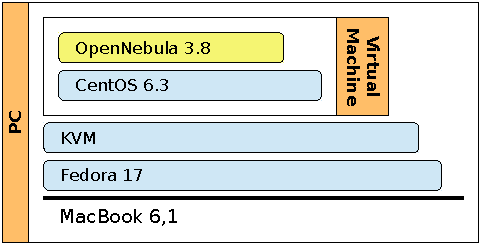
\includegraphics[width=0.55\textwidth]{imagenes/009.pdf}
 \caption{OpenNebula 3.8 con KVM}
\label{fig:opennebula}
\end{center}
\end{figure}

\begin{itemize}
 \item Se cre\'o una m\'aquina virtual soporte para todo el cloud OpenNebula: 1 GB RAM, 8 GB HDD, ACPI y APIC.
 \item Se descarg\'o, instal\'o y actualiz\'o CentOS 6.3.
 \item Se nombr\'o \emph{opennebula} a la m�quina virtual.
 \item Igualmente nombrado, se dio de alta un nuevo usuario, \emph{opennebula}, y se agreg\'o a la lista de \emph{sudoers}.
 \item Se detuvo \texttt{SELinux}.
 \item Se sigui\'o la gu\'ia contenida en \cite{centosonquickstart} para concluir el proceso, al que hubo que integrar las siguientes cuestiones para probar el framework:
  \begin{itemize}
   \item Por defecto, el servicio que brinda la interfaz web de OpenNebula (\texttt{sunstone}) se engancha en \emph{lo}. Para que pudiera ser accedido desde fuera del servidor, fuera de la m\'aquina virtual en este caso, fue necesario precisar que sunstone habr\'ia de escuchar en \emph{eth0}, modificando, para este fin, la configuraci\'on correspondiente en \texttt{/etc/one}. Lo mismo aconteci\'o con \texttt{occi}, el servicio REST de control del cloud.
   \item Adicionalmente, se agreg\'o a iptables la regla para no filtrar el tr\'afico en el puerto \texttt{9869}, el de sunstone inicialmente.
  \end{itemize}
\end{itemize}


\subsection{OpenStack}\label{subsec:openstack}
\noindent El caso de OpenStack es llamativo por varias razones. Representa la convergencia entre dos necesidades diferentes: la puramente computacional de la NASA y la orientada al almacenamiento de Rackspace. Complementariamente, tanto Red Hat como Canonical han sumado su aporte bajo la forma de scripts de instalaci\'on y control en el caso de Red Hat, y escribiendo utilidades de despliegue autom\'atico, como \texttt{juju}, en el caso de Canonical.\newline

Como en el caso de OpenNebula, se configur\'o un entorno de ejecuci\'on contenido en una sola m\'aquina virtual. En este caso se eligi\'o a Fedora frente a CentOS y Ubuntu por el soporte comunitario en forma de extensa gu\'ia de instalaci\'on r\'apida \cite{quickstartfedoraos} y por la existencia de herramientas que ace\-le\-ra\-r\'ian sustancialmente el procedimiento. La gu\'ia de instalaci\'on y despligue oficial de OpenStack Folsom \cite{installdeployosfolsom}, est\'a escrita centr\'andose excesivamente en Ubuntu, lo que se tradujo en comandos no aplicables en Fedora. Como \'ultimo comentario previo a la descripci\'on de la puesta en marcha, decir que se probaron dos versiones de OpenStack: \emph{Essex} y \emph{Folsom}. La raz\'on radica en el hecho de que, a pesar de ser Essex la soportada oficialmente por la distribuci\'on (Fedora 17), desde la gu\'ia r\'apida mencionada anteriormente \cite{quickstartfedoraos} se recomendaba usar la \'ultima versi�n de OpenStack disponible ---Folsom a diciembre de 2012---, habilitando un re\-po\-si\-to\-rio de avance a tal fin.\newline

El grado de madurez observado de Folsom frente a Essex es sustancialmente llamativo en la interfaz web: lo que parec\'ia una primera aproximaci\'on para formular comandos de administraci\'on del cloud, evolucion\'o hacia una interfaz mucho m\'as cohesionada con el comportamiento real. El ejemplo si\-guien\-te pone de manifiesto esta idea: en el momento de lanzar instancias para probar el correcto funcionamiento del cloud, se observ\'o que, en caso de existir alg\'un problema de configuraci\'on en el subsistema de red que impidiese que las instancias obtuviesen direcciones IP, \'estas permanec\'ian en un estado que hac\'ia imposible su eliminaci\'on desde la interfaz web. Fue necesario recurrir a la edici\'on de la base de datos y la estructura de ficheros del controlador del cloud, con algunos resultados nefastos como la p\'erdida de informaci\'on de uso de las instancias, para restablecer la coherencia en Essex. El mismo problema se solventa directamente en Folsom (tanto desde la interfaz web como desde la l\'inea de comandos).\newline

Siguiendo el \'indice siguiente se dispuso un entorno de ejecuci\'on id\'entico para sendas versiones (ver figura \ref{fig:openstack}).

\begin{figure}[tbp]
\begin{center}
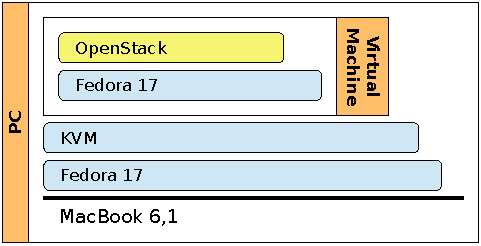
\includegraphics[width=0.55\textwidth]{imagenes/010.pdf}
 \caption{OpenStack en despligue virtual}
\label{fig:openstack}
\end{center}
\end{figure}

\begin{itemize}
 \item Se cre\'o una m\'aquina virtual para todo el cloud OpenStack: 1 GB RAM, 10 GB HDD, APIC y ACPI.
 \item Se descarg\'o, instal\'o y actualiz\'o Fedora 17.
 \item Se nombr\'o \emph{openstack} a la m\'aquina virtual.
 \item Igualmente nombrado, se dio de alta un nuevo usuario, \emph{openstack}, y se agreg\'o a la lista de \emph{sudoers}.
 \item Se instal\'o el paquete \texttt{acpid} para poder controlar los aspectos de energ\'ia desde el manejador de cloud.
 \item Se detuvo SELinux.
 \item Se orden\'o una copia en profundidad de la m\'aquina virtual ---tanto configuraci\'on de la m\'aquina como HDD--- para probar Essex y Folsom, y se renombraron convenientemente.
 \item Se siguieron tanto la gu\'ia de instalaci\'on r\'apida extraoficial \cite{quickstartfedoraos}, como la gu\'ia oficial de despliegue \cite{installdeployosfolsom}, dejando de lado la con\-fi\-gu\-ra\-ci\'on de \texttt{Swift}, para concluir el procedimiento.
 \item A mayores, se crearon sendos discos virtuales de 4 GB para albergar los vol\'umenes del almacenamiento de bloque gestionados por \texttt{Compute}, para Essex, y \texttt{Cinder} para Folsom.
\end{itemize}
 

\section{Conclusiones}\label{sec:conclusiones}
\noindent Presentamos, seguidamente, los resultados de la comparaci\'on de los frameworks de IaaS, atendiendo a las cuestiones resaltadas en la metodolog\'ia.
 
\begin{description}
 \item[Instalaci\'on:] Sin lugar a dudas OpenNebula se lleva la palma. La gu\'ia de instalaci�n es, con mucho, la m\'as corta y ligera de seguir. Acarrea, no obstante, el problema de tener un desconocimiento mayor de lo que est\'a sucediendo bajo la superficie, que dificultar\'a la resoluci\'on de los problemas que pudieran aparecer, as� como el manejo general del cloud.
 \item[Configuraci\'on y manejo:] El aprovisionamiento de nueva infraestructura, es decir, la uni\'on de nuevos anfitriones al cloud, requiere, en todos los frameworks analizados, la instalaci\'on en cada anfitri\'on del hipervisor que se pretenda utilizar. CloudStack y OpenNebula ofrecen una gesti\'on mucho m\'as transparente que OpenStack, siendo necesario ma\-yor esfuerzo de instalaci\'on y configuraci\'on. En este \'ultimo adem\'as, la interfaz web no deja forma alguna de conocer el tama\~no del cl\'uster real sobre el que corre el cloud ni, l\'ogicamente, el grado de utilizaci\'on de la infraestructura. Entre CloudStack y OpenNebula la diferencia es inexistente en cuanto a la funcionalidad expuesta a trav\'es de sus webs. CloudStack expone los servicios de todo el cloud como una jerarqu\'ia; OpenNebula como una tabla.
 \item[Hipervisor:] En cuanto a hipervisores soportados se refiere, OpenStack aventaja claramente a CloudStack y OpenNebula. Sin embargo, se podr\'ia afirmar que este hecho es pr\'acticamente anecd\'otico porque los tres soportan los m\'as conocidos ---KVM, Xen, variantes de Xen y variantes de VMWare--- que son los utilizados en casi todos los despliegues reales.
 \item[Almacenamiento:] Los tres soportan una m\'as que surtida variedad de controladores de \emph{backend} de datos. Pero, en este caso, es importante subrayar el esfuerzo de OpenStack por implementar la funcionalidad ofrecida por Amazon S3 ---almacenamiento en cloud r\'apido y seguro. Swift es el componente de OpenStack que otorga almacenamiento tolerante a fallos y de alta disponibilidad a los despliegues, sustent\'andose para lograrlo en la replicaci\'on y el balanceo de carga, entre otros. La gu\'ia avanzada de instalaci\'on de CloudStack \cite{cloudstackadvinstall}, muestra una primera aproximaci\'on para la configuraci\'on de Swift como almacenamiento secundario del cloud. De ah\'i se puede deducir en cierto grado la importancia y madurez de Swift como m\'odulo de OpenStack.
 \item[Documentaci\'on:] Ninguno de los tres puede presumir de manuales de instalaci\'on oficiales correctos al 100\%. Adem\'as, como se da la circunstancia de que cada framework ha ido madurando con grados de exposici\'on diferentes a las diversas distribuciones Linux, la cobertura que ofrecen para cada sistema operativo es muy heterog\'enea; hasta el punto de confundir, en alg\'un caso, los nombres de los m\'odulos cuyas funciones hay que invocar. Por ejemplo, ambos manuales de instalaci\'on de CloudStack ---r\'apida \cite{cloudstackadvinstall} y avanzada \cite{cloudstackquickinstall}--- se siguen m\'as correctamente usando CentOS como sistema operativo de base y XenServer como hipervisor. OpenStack dispone oficialmente de manuales de ins\-ta\-la\-ci\'on que soportan tanto derivados de Red Hat ---Fedora, CentOS, el propio Red Hat Enterprise Linux, etc.--- como de Debian ---Ubuntu, Debian, etc.--- sin embargo, al realizar el despliegue sobre Fedora se observ\'o que el nombre de los servicios documentados no se correspond\'ia con el nombre real; en Ubuntu no sucede tal cosa. De todas formas, las incorrecciones son nimias y la extensi\'on de la documentaci\'on es m\'as que suficiente para despliegues en producci\'on.
 \item[Comunidad:] A pesar de que pueda resultar algo secundario, la calidad del soporte comunitario es vital para el desarrollo y soporte de los frameworks. Todos ellos est\'an compuestos por m\'odulos escritos en c\'odigo abierto y libre en su mayor parte, de forma que, cuanto mayor sea el bullicio recogido en foros de desarrollo, mayor ser\'a tambi\'en el aporte recibido; y as\'i, el grado de madurez operativo, funcional y documental ser\'a mayor. A pesar de que no pueda darse un claro vencedor en este apartado, debido al car\'acter difuso de la magnitud \emph{soporte comunitario}, s\'i es interesante destacar el importante apoyo a OpenStack de Canonical y Red Hat: no hay conferencia o charla t\'ecnica general de uno u otro donde no hagan referencia a OpenStack.
\end{description}

\subsection{OpenStack Folsom}\label{subsec:openstackfolsom}
\noindent Finalmente, el framework para cloud IaaS elegido es OpenStack Folsom. Las gu\'ias de instalaci\'on mencionadas, el soporte comunitario, el empuje por parte de dos pesos pesados del software, los despliegues reales de HP, Dell, Intel, Rackspace, etc., la modularidad de configuraci\'on, la completitud de implementaci\'on (soporte de los APIs OCCI, S3, EC2 y definici\'on de un servicio de almacenamiento en cloud como Swift) y el soporte oficial de despliegue de prueba sobre m\'aquinas virtuales ---usando emulaci\'on--- han desequilibrado la balanza a su favor.

%\cleardoublepage
%\chapter{OpenStack Folsom}\label{cap:openstack}

\noindent The current section intends to detail the IaaS Cloud implementation that has been chosen: OpenStack. Initially, a global vision will be given to the reader, to progressively focus on its constituents modules' responsibilities and how they collaborate to maintain the service running.

\section{Global Architecture}\label{sec:arquitecturaglobal}

\noindent Figure \ref{fig:arquitecturaos} shows the three basic operational components of OpenStack Folsom:

\begin{description}
 \item[Functional Core:] OpenStack Compute, OpenStack Quantum and OpenStack Storage (Cinder and Swift).
 \item[Web Management Interface:] OpenStack Horizon.
 \item[Shared Services:] OpenStack Glance, OpenStack Keystone and other related services like a DBMS for persisting meta-data or a messaging queue.
\end{description}

\begin{figure}[tbp]
\begin{center}
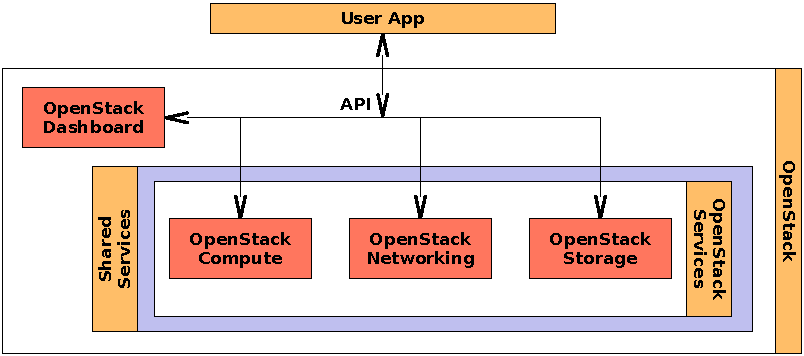
\includegraphics[width=0.9\textwidth]{imagenes/012.pdf}
 \caption{OpenStack Arquitecture}
\label{fig:arquitecturaos}
\end{center}
\end{figure}

The different components have been devised in a shared nothing fashion. This provides the cloud admin the flexibility required to distribute the modules over the cluster as pleased. An example of a particular OpenStack deployment is shown in figure \ref{fig:despliegueos}; OpenStack's own modules are displayed in red, supporting services are shown in violet. What it is missing from the diagram, for clarity, is the asynchronous queue that mediates inter-module communication. Qpid and RabbitMQ are the two queue implementations that are officially documented, being the former the one that we used in our test deployment.

\begin{figure}[tbp]
\begin{center}
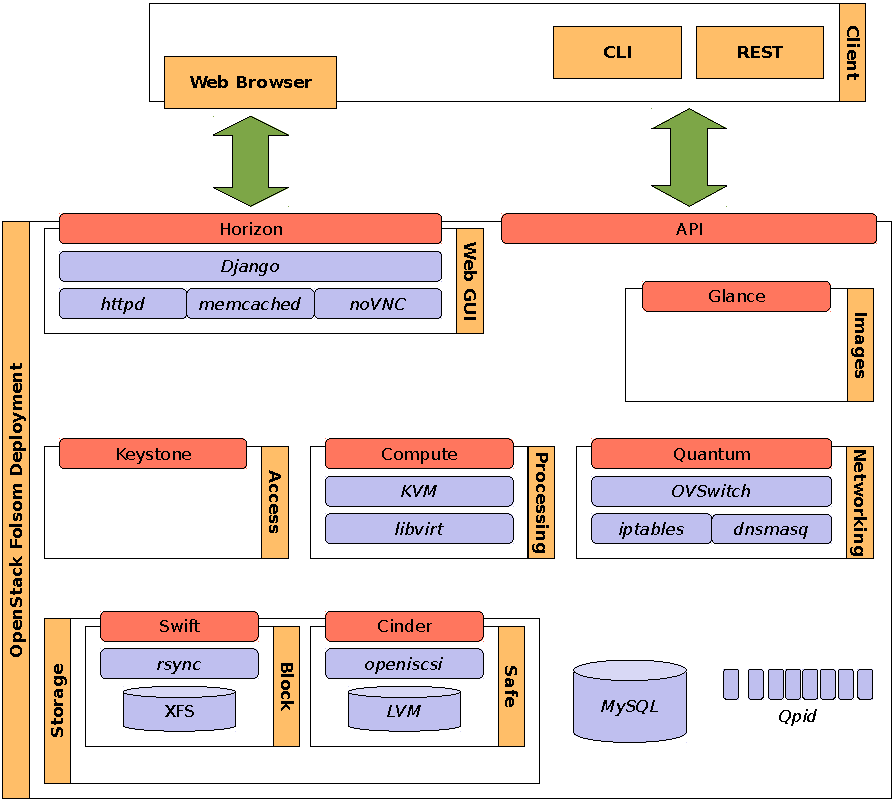
\includegraphics[width=0.99\textwidth]{imagenes/011.pdf}
 \caption{Example of an OpenStack Folsom deployment}
\label{fig:despliegueos}
\end{center}
\end{figure}

\section{Horizon}\label{sec:horizon}

\noident Horizon represents the fundamental window to set up the cloud. As discussed in the previous section, Horizon does not currently --- as of Folsom version --- present a global view of the physical infrastructure, leaving the user in the dark in this respect. Horizon is written in Python on top of \texttt{Django}, the web framework. Django itself relays on a web server like \texttt{httpd} to expose static files, uses a caching mechanism (\texttt{memcached}) to speedup load times and a terminal embedding (\texttt{noVNC}) system to view the output of the virtual graphic card directly on Horizon.

To manage and create instances in the cloud, OpenStack gives the cloud admin the ability to register authorization roles that will let the users consume those services whose role give access to. While the admin is allowed to sign up custom roles, two roles that ship the distribution are the \emph{Cloud Admin} and the \emph{Cloud Member}.

A user granted the admin role will be able to manage:

\begin{description}
 \item[Tenants:] Create, delete, member users, alter quotas, etc.
 \item[Users:] Create, modify or delete.
 \item[OS Images:] List, remove or modify meta-data.
 \item[Instances:] Reset, shutdown, suspend, print log on screen, etc.
 \item[Volumes:] Create, list, attach to an instance, etc.
 \item[Networks:] Create, modify or delete.
\end{description}

A user granted the member role will be able to:

\begin{description}
 \item[Status:] Quota, resources, etc.
 \item[Instances:] create, shutdown, reset, suspend, print log, create image from a running instance (snapshot), etc.
 \item[Volumes:] List, create, modify, attach to an instance, create a volume snapshot, etc.
 \item[Images:] Create, list, delete, modify, etc.
 \item[Networking:] Manage public IPs (floating IPs).
 \item[Security groups:] Create, delete or modify security rules.
 \item[Keypairs:] Create, modify or delete.
\end{description}

\section{Keystone}\label{sec:keystone}

\noindent Keystone is the central security check point and information repository storing information needed to access the cloud installed services. It verifies, before each request, user credentials and authorizations in OpenStack services. Keystone divides this functionality in two parts: on the one hand user control, on the other service catalog.

To deal with users, Keystone assigns them tenants or projects. Users, as discussed above, are granted the membership to a tenant and a service quota they will have to adhere to; they are also restricted to the tenant quota.

To organize the catalog at hand Keystone defines two other concepts within the service catalog: \emph{Services} and \emph{endpoints}. A service in the catalog is a mere abstract description of an exploitable cloud feature by the user. The particular implementation of the service is managed by the set of endpoints associated to it. Said collection contains every piece of information that is required for users to consume the services. Figure \ref{fig:secuenciais} shows a Sequence Diagram portraying the interchanged messages between the different entities taking part to consume a service: \emph{Create a new instance}.

\begin{figure}[tbp]
\begin{center}
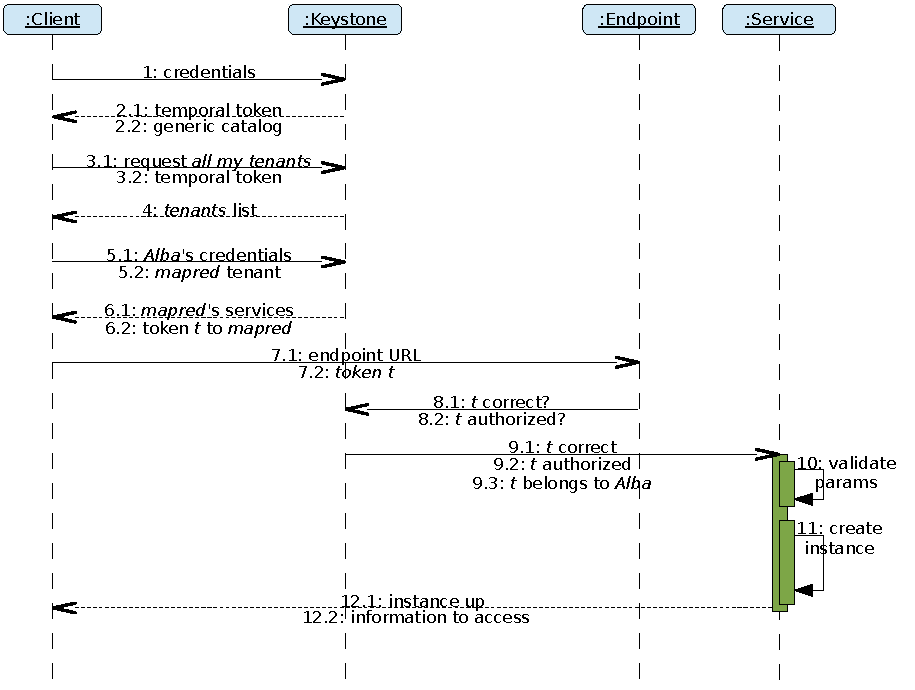
\includegraphics[width=0.99\textwidth]{imagenes/013.pdf}
 \caption{Sequence Diagram --- create instance}
\label{fig:secuenciais}
\end{center}
\end{figure}

Stemming from the fact that Horizon exposes only a part of OpenStack functionality, Keystone includes a CLI tool to interact with the REST service in charge of administrative operations to help dealing with administrative operations. Issuing certain commands to Keystone through a terminal requires the knowledge of the admin token, which has to be conveniently secured, or the login credentials of a user with the admin role. Lastly, it should be noted that Keystone uses a data base to store user access credentials and the service catalog meta-data.

\section{Quantum}\label{sec:quantum}

\noindent Starting in Folsom, Quantum is the module to manage virtual networking. It was introduced to separate the networking part from the computing part, held together in \texttt{Compute} module. Certainly, the fact that it had been refactored out demonstrates OpenStack's evolving model toward a more coherent less coupled functional allocation; and as it is independent, it could be configured in a dedicated node.

To bring virtual networking into existence Quantum banks on external plug-ins. Two of those plug-ins whose usage is covered in the official Quantum administrator manual (\cite{quantumadminfolsom}) are \texttt{OpenVSwitch} and \texttt{LinuxBridge}. Additionally, Quantum relies on iptables to configure routing rules and firewall, \texttt{dnsmasq} for the \emph{DNS}, the \emph{DHCP} and the \emph{NAT}.

Figure \ref{fig:desplieguequantum} pictures a topology example of a virtual network. On it, \emph{30.0.0.X} represent public IPs and \emph{10.0.X.Y} private. This virtual network assigns a virtual router to each tenant but more could be added with ease. Private IP overlapping over different networks is possible as expected (\emph{10.0.0.2}). The routers public IPs --- they could be assigned more external interfaces --- must be taken from the external network (\emph{30.0.0.0}).

\begin{figure}[tbh]
\begin{center}
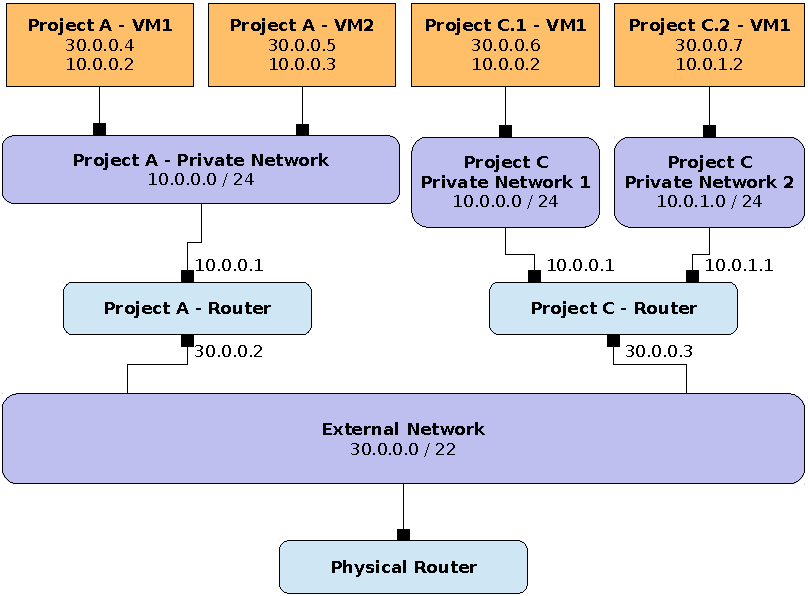
\includegraphics[width=0.9\textwidth]{imagenes/014.pdf}
 \caption{Virtual network deployment with Quantum}
\label{fig:desplieguequantum}
\end{center}
\end{figure}

\section{Compute}\label{sec:compute}

\noindent Compute is the central module. Its duty entails orchestrating the global workings in the cloud, delegating each particular function to the service on charge. In the end, Compute will let a logged user start virtual instances, which will draw their VCPU, VRAM and VHDD from the physical cluster. Yet required, Compute does not contain a virtualization package. The approach is to delegate infrastructure provision to a hypervisor found typically, but not restricted to, in the same node. To expose this on-demand computational service, Compute implements a REST API so that users can control their instances' life cycle directly from a REST client (like the CLI tools that accompany Compute).

To effectively create an instance, Compute will communicate with other modules within the cloud to orchestrate the execution and, finally, it will pass the request to the most suitable cluster node's hypervisor --- most suitable according to the cloud-defined rule set --- that will bring up the VM. Some of the supporting services are described bellow.

\begin{description}
 \item[Keystone:] Matches supplied vs. stored credentials, clearing or refusing requests.
 \item[Glance:] Finds the OS image that should be run.
 \item[Quantum:] Provides private and public IPs and checks network flow to/from the instance.
 \item[Cinder:] Drives block storage and so it is in charge of exposing \emph{hot-plugged} volumes into the instance.
 \item[Qpid:] Enables message passing among the different modules.
\end{description}

It has been said throughout the text that if there is a something aligning the differing IaaS implementations is their flexibility. Users' computational needs vary with time, so it seems reasonable to think they will expect their virtual services to adapt to them. Hypervisors have fulfilled this behavior since their design, making them ideal matches to help serve infrastructure as a service. OpenStack nomenclature --- inspired by AWS' --- calls each possible particular VM specification a \emph{flavor}.

Se ha venido diciendo a lo largo del texto que si algo alinea a los distintos cloud es su flexibilidad. Puesto que las necesidades computacionales de los usuarios var\'ian en funci\'on del tiempo, es necesario que, dentro de unos l\'imites, se les permita concretar las caracter\'isticas t\'ecnicas de las m\'aquinas virtuales. En OpenStack cada posible configuraci\'on instanciable, esto es, cada realizaci\'on concreta de la cantidad de recursos que temporalmente se expropian del anfitri\'on, se denomina \emph{flavor} ---siguiendo la nomenclatura de los AWS. De manera que se va a otorgar la posibilidad de que los usuarios autorizados puedan crear sus propios \emph{sabores} computacionales, definiendo el tama\~no del disco, el n\'umero de VCPUs, etc., sin ninguna dificultad, a trav\'es de Horizon.


\section{Glance}\label{sec:glance}
\noindent Glance es el servicio de hospedaje de im\'agenes para OpenStack. Se pueden configurar m\'ultiples backends de datos para guardarlas como: Swift, Amazon S3, el sistema de ficheros local o una ubicaci\'on HTTP; lo que mantiene el nivel de flexibilidad a la par con los dem\'as m\'odulos. Glance se vale de Keystone para manejar el acceso y la seguridad de las im\'agenes y se comunica con Compute para ponerlas en ejecuci\'on bajo demanda.
Ofrece soporte a una buena variedad de clases de im\'agenes y formatos de su contenedor; pero este hecho es meramente informativo para el cloud, ya que la capacidad o incapacidad de arrancar una instancia est\'a vinculada al hipervisor desplegado y no a Glance. Tambi\'en est\'a presente la habilidad de asociar metadatos a las im\'agenes en forma de pares \texttt{(clave, valor)}. Esta metainformaci\'on se utiliza para diferenciar distintas im\'agenes o para configurar el \emph{direct kernel boot} necesario para redimensionar el volumen ra\'iz al arrancar las im\'agenes en distintos sabores.


\section{Almacenamiento}\label{sec:almacenamiento}
\noindent OpenStack otorga tres opciones a la hora de elegir el tipo de almacenamiento:
\begin{description}
 \item[Vol\'atil:] las dimensiones del disco r\'igido sobre el que se dispone la ra\'iz del \'arbol de ficheros se fijan, en el momento de arrancar la m\'aquina virtual, a las marcadas por el sabor elegido. Los archivos contenidos en \'el son aquellos que aparecen en la definici\'on de la imagen del sistema almacenada en Glance. Las alteraciones de este sistema de ficheros no persisten entre ejecuciones de las instancias. Al ordenar la finalizaci\'on de la ejecuci\'on de un servidor virtual, se destruye el fichero temporal que reflejaba las modificaciones del usuario a dicho sistema de ficheros en esa ejecuci\'on concreta.
 \item[Persistente:] vali\'endose de vol\'umenes de almacenamiento gestionados por Cinder con ayuda de \emph{LVM} (\emph{Logical Volume Manager}), OpenStack otorga la posibilidad de enganchar a las instancias, en caliente, vol\'umenes l\'ogicos de tama\~nos indeterminados y creados bajo demanda. Con este tipo de salvaguarda, se garantiza que la informaci\'on no se pierde al terminar la sesi\'on de ejecuci\'on. Sin embargo, este mecanismo de almacenamiento tiene una importante limitaci\'on y es que no es posible enganchar un mismo volumen l\'ogico a dos instancias al mismo tiempo. La alta disponibilidad o la seguridad de la informaci\'on ante fallo no est\'an implementadas directamente, ya que los datos van a residir en un \'unico punto. Podr\'ian superarse estas limitaciones definiendo alguna pol\'itica de copia de seguridad o alguna cofiguraci\'on \emph{RAID} (\emph{Redundant Array of Idependent Disks}) sobre los vol\'umenes ---no recomendable porque OpenStack cuenta con un m\'odulo a tal fin (Swift).
 \item[Seguro:] OpenStack Swift es el m\'odulo que permite la gesti\'on autom\'atica del almacenamiento distribuido de forma segura y permitiendo despliegues para alta disponibilidad. Utiliza la replicaci\'on controlada para establecer el marco de seguridad y la alta disponibilidad, combatiendo as\'i los problemas derivados de la fragilidad inherente a los discos duros. Swift se escuda en \texttt{rsync} para sincronizar las r\'eplicas sobre particiones \emph{XFS}.
\end{description}


\subsection{Cinder}\label{subsec:cinder}
\noindent Cinder es el m\'odulo de OpenStack que maneja los dispositivos virtuales de almacenamiento en bloque; de funcionalidad similar a la del \emph{EBS} (\emph{Elastic Block Storage}) de Amazon. Cinder utiliza una implementaci\'on de \emph{iSCSI} (\texttt{open-iscsi}) y LVM para Linux para gestionar las operaciones sobre los vol\'umenes. La creaci\'on, el enganche y desacople y el borrado de los bloques de almacenamiento persistente se maneja desde Horizon directamente.\newline

Estos bloques virtuales de persistencia se gestionan como vol\'umenes l\'ogicos pertenecientes a un grupo de vol\'umenes controlado por Cinder. Cinder no pretende crear un medio compartido como \emph{NFS} (\emph{Network File System}), o alguna soluci\'on \emph{SAN} (\emph{Storage Area Network}) o \emph{NAS} (\emph{Network Attached Storage}) para las instancias, ya que no es posible compartir un mismo vo\-lu\-men l\'ogico con m\'as de una m\'aquina virtual en un mismo instante. Una opci\'on interesante, que permite Cinder para facilitar ciertos despligues virtuales heterog\'eneos, es configurar las instancias para que arranquen desde un volumen creado por Cinder.


\subsection{Swift}\label{subsec:swift}
\noindent Al igual que suced\'ia con Cinder, Swift tampoco se enmarca en la idea tradicional de almacenamiento compartido en red, ni debe compararse con el anterior; Cinder y Swift cubren demandas diferentes. Se dice que Swift es ``\textit{un sistema escalable de almacenamiento de objetos, donde los usuarios registrados controlan sus compartimentos de datos o contenedores, subiendo, descargando o borrando ficheros a su antojo}'' \cite{osswift}. Funcionalmente Swift equivale al S3 de Amazon y al \texttt{Walrus} de Eucalyptus, siendo posible con\-fi\-gu\-rar un API REST compatible, parcialmente por el momento (enero 2013), con la sintaxis del primero. Una caracter\'istica fundamental para Swift es la replicaci\'on controlada.


\subsubsection{Replicaci\'on}\label{subsubsec:replicacion}
\noindent La escalabilidad, la tolerancia a fallo, la alta disponibilidad, la seguridad, el balanceo de almacenamiento y el control de carga son algunos de los rasgos que definen a Swift. La alta disponibilidad y la tolerancia a fallo se implementan usando la replicaci\'on. La replicaci\'on es un mecanismo a trav\'es del cual un sistema distribuido mantiene copias o \emph{r\'eplicas} en puntos diferentes de su despliegue, para mejorar sus prestaciones o limitar el alcalce de los fallos, entre otros.\newline

En Swift, los procesos de replicaci\'on de cada \emph{Servidor de Objetos}, que es un nodo cualquiera del cl\'uster con Swift en funcionamiento, van a comparar, peri\'odicamente, sus copias locales con cada copia remota para verificar su grado de actualizaci\'on. Cotejar estas r\'eplicas es un proceso tan costoso computacionalmente como habitual en sistemas de almacenamiento distribuido, por eso Swift se vale de estructuras como las \emph{listas Hash} o las \emph{marcas de agua} para acelerar las comparaciones. Rsync o HTTP gestionan la trans\-fe\-ren\-cia de las copias en funci\'on del tipo de objeto a replicar. La transparencia de replicaci\'on es uno de los pilares que soportan la escalabilidad de Swift. Cuando se a\~nade un nuevo nodo al espacio de almacenamiento de Swift, la redistribuci\'on de las copias es autom\'atica y, desde el momento en que \'este sea sincronizado, podr\'a responder a peticiones de datos de los usuarios.

\subsubsection{Updaters y Auditors}\label{subsubsec:otroscompswift}
\noindent Otros componentes interesantes, que completan el c\'irculo funcional descrito para Swift, son los \emph{Updaters} y los \emph{Auditors}. Los primeros act\'uan cuando se produce un error de sincronizaci\'on entre copias o cuando la carga computacional de un Servidor de Objetos es lo suficientemente alta como para que no pueda satisfacer una operaci\'on. Sucede entonces que la ejecuci\'on de esa operaci\'on se difiere; se a\~nade a una cola de actualizaci\'on que el Updater va procesando para restablecer la sincronizaci\'on. Los Auditors escanean continuamente el sistema de ficheros en busca de fallos de integridad en objetos, contenedores o cuentas de usuario, tal que, si encontrasen incoherencias, pondr\'ian en cuarentena a la entidad y pedir\'ian que se estableciese una nueva r\'eplica.

%\cleardoublepage
%\chapter{Hadoop}\label{cap:hadoop}
\noindent This chapter tries to expose with simplicity the defining fundamentals of Hadoop architecture. Initially abstract concepts will be introduced to give way to more particular and deep ideas that explore Hadoop implementation of the MapReduce model in two layers: the processing and the storage subsystem.

\section{The Beginnings}\label{sec:origen}
\noindent Hadoop roots its origins in \emph{Apache Nutch}, Mike Cafarella and Doug Cutting's implementation of an open source web index and search engine. Nutch project began in 2002. In spite of the Internet being notoriously smaller at the time, Nutch's underlying technology was unable to make it scale to manage the billion pages that comprised the \emph{old} Internet. But in 2003 Google publishes a research paper introducing \emph{GFS} (\emph{Google File System}) \cite{gfs}, a file system to be used across their clusters of commodity pcs that greatly simplified its deployment. Nutch will inherit a large part of the concepts detailed there translated in their own distributed file system implementation (\emph{NDFS}).

Also in 2004 appeared another publication \cite{googlemapreduce} that presented MapReduce, bringing about successive efforts to port Nutch algorithms to adapt to the emerging model. In mid 2005 most of Nutch code run following MapReduce guidelines over NDFS.

Both NDFS and Nutch MapReduce implementation were generic enough to be used without refactoring beyond web page indexing. In 2006 an unrelated project was constituted to extend Nutch's potentially reusable parts to widen their applicability context. This project was called Hadoop. In 2008 \emph{Yahoo!} announced that the index for their search engine in production was being continually refreshed by 10,000 Hadoop nodes. This same year Hadoop is brought out to the world becoming an Apache-backed project corroborating its success.

Nowadays, Hadoop is without doubt the MapReduce implementation most widely used by a broad range of companies.

\section{General Hadoop Architecture}\label{sec:arquitecturahadoop}
\noindent Hadoop composition differentiates four modules:
\begin{description}
 \item[Hadoop Common:] A module containing the parts used across the implementation. It is mainly comprised of scripts and configuration tools.
 \item[Hadoop MapReduce:] The module implementing the MapReduce processing model.
 \item[Hadoop YARN:] A general purpose framework abstracted from Hadoop MapReduce. It is employed to manage resources and schedule executions in distributed environments.
 \item[Hadoop DFS:] The distributed file system sustaining inputs and outputs from Hadoop clusters.
\end{description}

Hadoop architecture corresponds to the \emph{Master-Worker} archetype where two roles on each cluster appear: a unique Master and various Workers. These roles, and thus responsibilities, are fixed to different nodes by the cluster admin. If necessary, e.g. for maintenance, the admin may freely re-set the roles to new cluster nodes, only requiring job resubmissions if the Master role were reassigned.

This section will almost exclusively center around MapReduce and Hadoop DFS (HDFS) modules to expose the functionally covered with Hadoop. Hadoop YARN, as discussed, is a subsystem resulting from the isolation of scheduling and processing, both found together in the old --- pre Hadoop 2 --- MapReduce module, retaining task distribution and planning within YARN. This way, YARN is allowed to untie from Hadoop allowing for deployments where YARN orchestrates an implementation-agnostic working set. As of this writing, Hadoop YARN is still an alpha version.

Figures \ref{fig:hadoopmapredhdfs} and \ref{fig:hadoopmapreddfs} exhibit a high level vision of Hadoop architecture. Figure \ref{fig:hadoopmapredhdfs} shows an hypothetical deployment with HDFS. Figure \ref{fig:hadoopmapreddfs} shows a particular Hadoop installation with another supporting distributed file system.

\begin{figure}[tbp]
\begin{center}
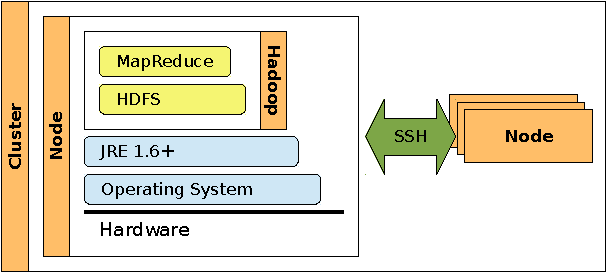
\includegraphics[width=0.7\textwidth]{imagenes/015.pdf}
 \caption{Hadoop over HDFS}
\label{fig:hadoopmapredhdfs}
\end{center}
\end{figure}

\begin{figure}[tbp]
\begin{center}
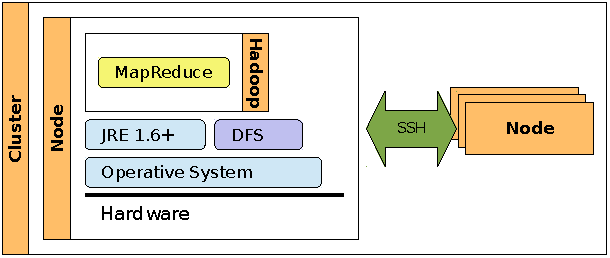
\includegraphics[width=0.7\textwidth]{imagenes/016.pdf}
 \caption{Hadoop over another DFS}
\label{fig:hadoopmapreddfs}
\end{center}
\end{figure}

From the figures it can be deduced that Hadoop runs atop a \emph{Java Virtual Machine} (emph{JVM}), that MapReduce requires a DFS implementation to rely on and that inter-node communication is conveyed through \emph{SSH} tunnels over TCP. Every module includes a web server (\emph{Jetty}) to ease collecting and reporting status information.

\section{Hadoop Distributed File System}\label{sec:hdfs}
\noindent HDFS has been designed to act as archival repository for huge masses of data whose main access pattern be \emph{write-one} \emph{read-many}. While it is no requisite for a data query to follow this access pattern, HDFS performance shines with read queries in batch mode. The underlying infrastructure, again, is composed by commodity pcs that HDFS manages to transform into a reliable, scalable, fault tolerant, self-balancing and network traffic reducing data store. Yet, as individual nodes are regular pcs, in HDFS converge some operating limitations:

\begin{itemize}
 \item High data access time. HDFS prioritizes large reads in batches and thus, reading small files is generally discouraged. As complement though, HDFS delivers \emph{very} high throughput by leveraging parallel reads on the cluster.
 \item High data writing time on many small files. Writing a file changes a block. Every file that be smaller than the HDFS block size must be persisted in a single block. That changed block must be send out across the network to keep the file system consistently updated. Thus, appending to many files requires updates in many blocks that would require synchronizing over the network.
 \item Multiple writes to the same file or ``\emph{not-append}'' operations are not supported. HDFS is not a \emph{POSIX}-compilant file system implementing only a set of operations to try to maximize data throughput in distributed environments.
\end{itemize}

To organize storage, HDFS takes from traditional operating systems the concept of block: an abstraction of the particular drive structure with a double purpose:

\begin{description}
 \item[Lowering DFS complexity:] Writing a block comprises storing data and meta-data, and handling information related to locate those data on disk. Using the block as the minimum organizational structure simplifies location expressions.
 \item[Incrementing flexibility:] files are free to grow over the size of an HDFS block.
\end{description}

To lay local drive blocks in position, HDFS makes use of two processes: the \emph{DataNode} and the \emph{NameNode}. Besides, as support, from Hadoop 0.21.0 onward it is permitted the optional deploying of a \emph{Backup Node} and a \emph{Checkpoint Node} in the same cluster.

\subsection{Node Roles}\label{subsec:rolesnodos}
\noindent Figure \ref{fig:desplieguehdfs} shows a layered down HDFS deployment. In dotted line appear both the Backup Node and the Checkpoint Node.

\begin{figure}[tbp]
\begin{center}
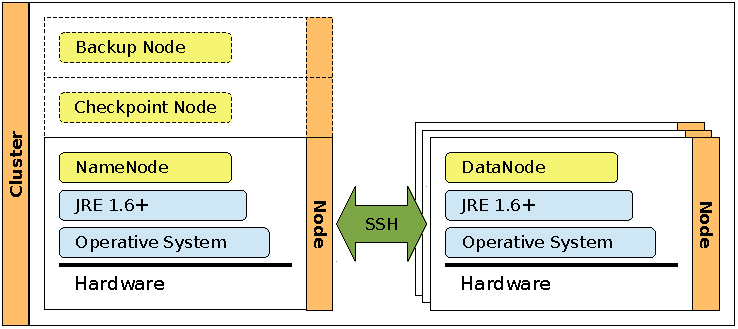
\includegraphics[width=0.85\textwidth]{imagenes/017.pdf}
 \caption{Typical HDFS deployment}
\label{fig:desplieguehdfs}
\end{center}
\end{figure}

\subsubsection{DataNode}\label{subsubsec:datanode}
\noindent DataNodes are those processes within nodes that handle the storage of HDFS blocks in their local drives. Every time a write to a file in a block succeeds, the DataNode in charge of the operation signals its supervising NameNode so that it could keep track the modifications to the DFS as they happen.

\subsubsection{NameNode}\label{subsubsec:namenode}
\noindent The NameNode is the process appointed to deal with the name space of the cluster. It has to handle the file system tree and meta-data that make possible recovering data from the DFS. It is such an important process that if it went down, every piece of data in HDFS would get lost, rendering impossible to match files with their container blocks. Therefore, the NameNode is seldom deployed with no Checkpoint Nodes or Backup Nodes in case the HDFS data were not stored elsewhere.

The information about the file system, meta-data, is persisted to the NameNode both in memory and disk. In this latter form, meta-data is managed in two files: one contains the name space of the file system as an image (\texttt{fsimage}), the other progressively appends the changes to the fsimage (\emph{edits}) as a log. When the DataNode starts, it compiles an fsimage afresh by merging the existing fsimage with the edits file. As soon as changes to the HDFS are reported from the NameNodes, the DataNode will update the edits log but without touching the fsimage. In a typical secured deployment, the edits file is kept in memory within the NameNode host computer, on the local file system and remotely via NFS.

\subsubsection{Checkpoint Node}\label{subsubsec:checkpointnode}
\noindent El fin que se persigue agregando un nodo de este tipo es mitigar los problemas relacionados con la ca\'ida de operaci\'on del NameNode. Peri\'odicamente, el Nodo de Checkpoint va generando puntos de restauraci\'on, o \emph{checkpoints}, siguiendo la misma estrategia que en el NameNode, es decir, usando \texttt{fsimage} y \texttt{edits}. Cada cierto tiempo, se descargar\'an ambos ficheros desde el NameNode y se fundir\'an, formando una nueva imagen actualizada que ser\'a transferida al NameNode. Cuando haya finalizado con \'exito la operaci\'on, el NameNode tendr\'a que purgar la imagen antigua e iniciar un nuevo fichero de log que albergue los cambios que se vayan sucediendo.


\subsubsection{Backup Node}\label{subsubsec:backupnode}
\noindent El Nodo de Backup provee la misma funcionalidad de generaci\'on de puntos de restauraci\'on que el Checkpoint Node pero usando una aproximaci\'on diferente. Para mantener sincronizado su espacio de nombres con el del NameNode que plagia, este tipo de nodo se descarga el \texttt{fsimage} al arrancarse y lo actualiza con las modificaciones que vaya captando el NameNode. Adicionalmente y cada cierto tiempo, el Backup Node actualiza su \texttt{fsimage} con los \texttt{edits}, creando un punto de restauraci\'on asociado.\newline

En comparaci\'on con el Checkpoint Node, este nodo consume menos ancho de banda de red ya que no necesita descargarse el \texttt{fsimage} y los \texttt{edits} del NameNode para mantener el sincronismo de estado.\newline

Como apuntes finales, destacar que de momento (versi\'on 1.0.4 de Hadoop), s\'olo se soporta un Nodo de Backup por NameNode o m\'ultiples Nodos de Checkpoint, y que la presencia de un Backup Node habilita la posibilidad de correr el NameNode sin almacenamiento persistente, delegando esa res\-pon\-sa\-bi\-li\-dad al Nodo de Backup.


\subsection{Topolog\'ia de red}\label{subsec:topologiared}
\noindent Una de las partes fundamentales de un sistema de ficheros en un entorno distribuido es proveer al usuario de un mecanismo transparente, que garantice la persistencia de la informaci\'on en \'el contenida manteniendo un cierto nivel de prestaciones. El HDFS utiliza una t\'ecnica, ya citada para los cloud, la replicaci\'on, que proporciona altas prestaciones, escalabilidad y tolerancia a fallo, al tiempo que limita la congesti\'on de red controlando la ubicaci\'on y el n\'umero de copias de los bloques en el centro de datos.

\subsubsection{Distancia entre nodos}\label{subsubsec:distnodos}
\noindent Para poder soportar las prestaciones comentadas, es fundamental que el NameNode, que es quien gestiona la distribuci\'on de las r\'eplicas de los bloques, tenga cierto conocimiento de la organizaci\'on f\'isica de los nodos que participan en el despliegue. La idea fundamental es tratar de mantener un equilibrio en la separaci\'on de las copias, entendida como la \emph{distancia f\'isica} entre los nodos que almacenan cada una: la distancia media entre r\'eplicas es proporcional tanto a la tolerancia a fallo del sistema, como al ancho de banda consumido para enviar cada r\'eplica. Recordemos que el ancho de banda de red disponible para transferir informaci\'on entre distintos nodos se reduce a medida que los alejamos, o visto de desde otro \'angulo, que la transferencia ser\'a m\'as costosa cuanto mayor sea la distancia entre el nodo que contenga el bloque original y aquel que vaya a albergar la r\'eplica. Es decir, ser\'ia id\'oneo, para equilibrar la separaci\'on entre r\'eplicas, definir una m\'etrica que calculase la distancia entre dos nodos cualesquiera.\newline

Como los nodos de las redes IP siguen una estructura de \'arbol invertido, y la red de un cl\'uster Hadoop es de este tipo, se podr\'ia considerar, como aproximaci\'on de la distancia f\'isica entre nodos, la \texttt{distancia internodal}: \emph{la suma de las distancias de los nodos al ancestro com\'un m\'as pr\'oximo}.\newline

Tal y como se ha comentado, HDFS utiliza RPC sobre TCP/IP a trav\'es de SSH para la comunicaci\'on entre nodos, lo cual (capa IP) no aporta informaci\'on de localizaci\'on \emph{concreta} de cada nodo dentro del despliegue. Para concretar la distancia internodal y as\'i poder hacer un reparto \'optimo de las copias, es necesario configurar HDFS para que cada IP sea mapeada a una posici\'on concreta, de tantas componentes ---\texttt{(centro de datos, rack, nodo)}, por ejemplo--- como niveles haya en la red. La figura \ref{fig:distnodos} muestra un ejemplo con los valores m\'as comunes de la distancia internodal. Veremos c\'omo se calcula para el caso \texttt{d=4}.\newline

Fij\'andonos en la figura \ref{fig:distnodos}, el bloque azul representa la copia original, y el bloque amarillo, destino del arco azul con etiqueta \texttt{d=4}, la r\'eplica. Ambos bloques se encuentran en nodos de distintos racks en el mismo centro de datos. El ancestro com\'un m\'as pr\'oximo entre ellos ser\'a el enrutador que maneje el tr\'afico entre ambos racks. Adem\'as, cada nodo tiene que atravesar otro enrutador de rack, otro ancestro m\'as pr\'oximo a los nodos, que dirige la paqueter\'ia dentro del rack. Con lo que tenemos \emph{dos pasos} (distancia 2) para llegar al router que conecta ambos racks por cada nodo; sumando ambas distancias obtenemos el resultado.

\begin{figure}[tbp]
\begin{center}
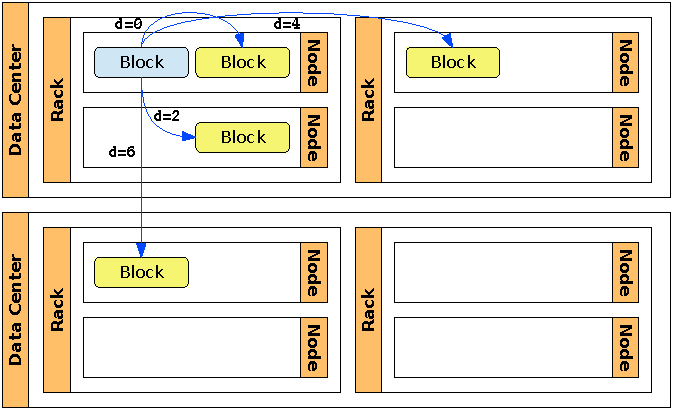
\includegraphics[width=0.75\textwidth]{imagenes/018.pdf}
 \caption{Ejemplo de valores de distancias internodales}
\label{fig:distnodos}
\end{center}
\end{figure}



\subsubsection{Replicaci\'on}\label{subsubsec:replicacionbloques}
\noindent La replicaci\'on es una t\'ecnica transparente al usuario y controlada por el NameNode que, para ser explotado en \'optimas condiciones, deber\'ia tener conocimiento de la distancia internodal. El grado de separaci\'on entre dos r\'eplicas es directamente proporcional al grado de robustez que aporta la copia ---la tolerancia a fallo--- e inversamente proporcional a la eficiencia de transmisi\'on por red, puesto que el ancho de banda disponible para mover un bloque entre dos centros de datos, ser\'a menor que para gestionar la r\'eplica de modo local al nodo, como ya hemos indicado. De tal manera que si se produjese la ca\'ida de un computador, la probabilidad de propagaci\'on de esa ca\'ida disminuye a medida que nos alejamos del nodo problem\'atico ---imaginemos una inundaci\'on del centro de datos, por ejemplo.\newline

La estrategia concreta que sigue HDFS consiste en colocar la primera r\'eplica en el mismo nodo que el cliente del sistema de ficheros, si \'este pertenece al cl\'uster de almacenamiento ---una aplicaci\'on cliente corriendo en un nodo del cl\'uster HDFS, por ejemplo. En caso de que el cliente sea externo al cl\'uster, se elige un nodo al azar, teniendo en cuenta su carga computacional ---prio\-ri\-zan\-do los de menor carga. La segunda r\'eplica se coloca fuera del rack en el que se encuentre la primera copia; el rack concreto se elige al azar. La tercera se emplaza en el mismo rack que la segunda copia pero en un nodo diferente, de nuevo eligiendo al azar y balanceando carga. Las r\'eplicas sucesivas ---el factor de replicaci\'on se controla en el fichero de despliegue de HDFS--- se env\'ian a nodos, siempre diferentes, de este \'ultimo rack.\newline

La mec\'anica descrita aporta el equilibrio deseable entre tolerancia a fallo (ya que habr\'a copias de cada bloque en dos racks distintos), ancho de banda consumido (ya que la escritura de cada bloque s\'olo atraviesa un \emph{switch} o enrutador y las copias sucesivas se hacen dentro del mismo rack), rendimiento de lectura (al poder elegir entre dos racks ante cada petici\'on de lectura de un bloque) y distribuci\'on equilibrada de los bloques en el cl\'uster (que realiza HDFS al ejecutar el m\'etodo descrito). La figura \ref{fig:repbloque} muestra un ejemplo de replicaci\'on con factor 3 en un solo centro de datos. El n\'umero entre corchetes indica el orden de creaci\'on de cada copia; el bloque original, recientemente actualizado o creado, es el azul.

\begin{figure}[tbp]
\begin{center}
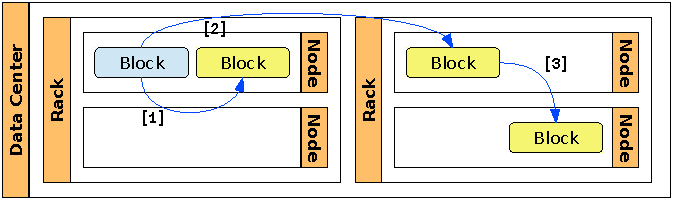
\includegraphics[width=0.75\textwidth]{imagenes/019.pdf}
 \caption{Ejemplo de replicaci\'on de un bloque, factor 3}
\label{fig:repbloque}
\end{center}
\end{figure}


\section{Hadoop MapReduce}\label{sec:hadoopmapred}
\noindent En un cl\'uster t\'ipico sobre HDFS se dispone la capa de operaci\'on de Hadoop, Hadoop MapReduce, que lleva a cabo la ejecuci\'on de los trabajos de mapeo y reducci\'on enviados al framework. Habiendo ya introducido las bases del paradigma MapReduce, corresponde ahora especificar aquellas desviaciones concretas de la implementaci\'on en Hadoop. Como era esperable, Hadoop MapReduce se basa en los principios expuestos en el art\'iculo de Google \cite{googlemapreduce} en cuanto a reparto de tareas y gesti\'on de fallos. Su arquitectura de alto nivel no dista mucho de la observada en la capa HDFS y as\'i se distinguen los roles \emph{maestro} y \emph{esclavo}.\newline

Por una parte, aparece el \emph{JobTracker}, encargado de planificar el reparto de las tareas a los nodos del cl\'uster; por la otra, el \emph{TaskTracker}, que ejecuta las tareas en los nodos como funciones Map y Reduce.\newline

Igual que su sistema de ficheros distribuido, Hadoop MapReduce est\'a escrito en Java.


\subsection{Roles de los nodos}\label{subsec:rolesnodosmapred}
\noindent La figura \ref{fig:desplieguehadoopmapred} representa un despliegue t\'ipico de Hadoop MapReduce en un cl\'uster, utilizando HDFS como sistema de ficheros distribuido soporte. Para completar la \emph{fotograf\'ia} habr\'ia que incluir los nodos responsables de gestionar el HDFS ---NameNode, Checkpoint Node y Backup Node--- omitidos por claridad.

\begin{figure}[tbp]
\begin{center}
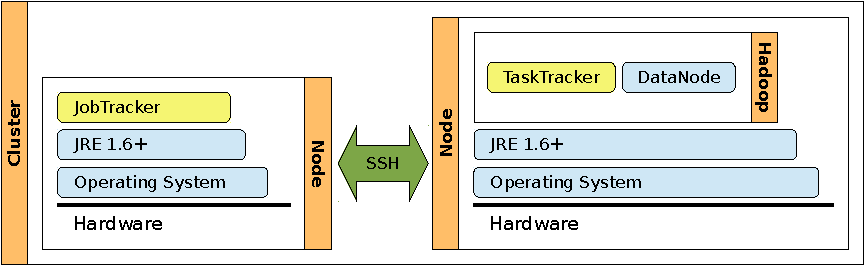
\includegraphics[width=0.99\textwidth]{imagenes/020.pdf}
 \caption{Ejemplo de despliegue de Hadoop MapReduce}
\label{fig:desplieguehadoopmapred}
\end{center}
\end{figure}

\subsubsection{JobTracker}\label{subsubsec:jobtracker}
\noindent El comportamiento del nodo JobTracker es muy similar al expuesto en el caso del NameNode de HDFS, pero aplicado a la gesti\'on de trabajos y tareas. Ante una petici\'on de ejecuci\'on, el JobTracker dividir\'a el trabajo asociado en tareas que repartir\'a entre los TaskTrackers que tenga bajo supervisi\'on. Normalmente, el tama\~no de los ficheros de entrada de las tareas se hace coincidir con el de los bloques del sistema de ficheros distribuido, sea o no HDFS, por ser lo m\'as eficaz. Para cerciorarse de que las ejecuciones concluyen con \'exito en un entorno expuesto al fallo, el JobTracker mantiene una lista de estado de las tareas asociadas a los nodos TaskTracker. De tal forma, en caso de que se produjese un error que impidiese la finalizaci\'on de alguna tarea, ya sea una tarea Map o una Reduce, el JobTracker replanificar\'ia su ejecuci\'on en otro nodo disponible con la m\'inima carga computacional.\newline

El reparto de trabajo se lleva a cabo siguiendo la m\'axima localidad, esto es, haciendo que los TaskTrackers reduzcan tareas basadas en la transformaci\'on de datos almacenados en el mismo nodo. As\'i se reducen tanto el tiempo de acceso al dato del TaskTracker, como la saturaci\'on de la red del cl\'uster, haciendo la computaci\'on m\'as ligera.\newline

Tal y como suced\'ia en la definici\'on general del MapReduce de Google \cite{googlemapreduce}, el fallo en un JobTracker es muy problem\'atico porque s\'olo est\'a cubierta la posibilidad de correr uno por cl\'uster sin usar herramientas adicionales. Dada una ca\'ida en el JobTracker, el procedimiento de recuperaci\'on ``resuelve'' la situaci\'on descartando los trabajos sin concluir; esperando que el nuevo JobTracker pueda hacerse cargo del procesado de esos trabajos incompletos que habr\'an de ser enviados manualmente por los usuarios. Actualmente s\'i se pueden manejar JobTrackers adicionales en un mismo cl\'uster e instante temporal usando una herramienta adicional: \emph{Zookeeper}.


\subsubsection{TaskTracker}\label{subsubsec:tasktracker}
\noindent La misi\'on fundamental del TaskTracker es procesar las tareas que le sean enviadas desde el JobTracker. Peri\'odicamente, el TaskTracker env\'ia una se\~nal a su JobTracker para informar acerca del estado de progreso de la ejecuci\'on de una tarea, si tuviese una asignada, o para indicar que se encuentra a la espera. Si el JobTracker no recibiese esa se\~nal en un intervalo convenido, \'este marcar\'ia el TaskTracker y \emph{todas} sus tareas relacionadas ---las concluidas y las incompletas--- como inaccesibles. Esta clase de fallo, es decir la ca\'ida de un TaskTracker, se considera menos problem\'atico que en el caso del JobTracker, pero implica replanificaci\'on de tareas e incluso repetici\'on de la ejecuci\'on de alguna. Usando la comentada lista de estado de las tareas, el JobTracker buscar\'a las inaccesibles necesarias ---las Map completadas y las Reduce cuya salida no est\'e en el DFS--- y har\'a la redistribuci\'on siguiendo la mec\'anica descrita.

%\cleardoublepage
%\chapter{A Private Cloud for MapReduce Applications}\label{cap:solucion}
\noindent This chapter introduces a novel solution combining the virtual infrastructure managed with OpenStack and the Hadoop implementation of MapReduce to conform a powerful computational tandem. \emph{qosh}, as this project has been called, will be described along this section moving from architecture to implementation.

\section{Architecture}\label{sec:diseno}
\noindent Figure \ref{fig:arquitecturaglobal} shows a high level portrait of qosh execution environment. The component that acts as interface between system and user is displayed on the right end. It abstracts the inherent difficulty in configuring the job execution context and in deploying the virtual cluster. Furthermore, qosh will keep track of submitted jobs, MapReduce \texttt{jar} files, input data and output results, with no need to walk the HDFS to search for data.

\begin{figure}[tbp]
\begin{center}
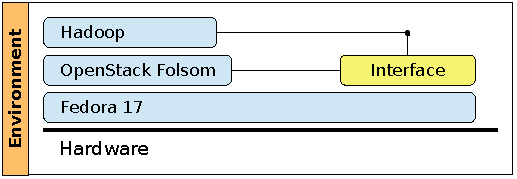
\includegraphics[width=0.65\textwidth]{imagenes/021.pdf}
 \caption{Global Architecture}
\label{fig:arquitecturaglobal}
\end{center}
\end{figure}

To streamline development, it is determined that the very first qosh version be tested on a personal computer. As shown on figure \ref{fig:arquitecturaglobal}, Fedora Linux is installed atop the hardware and OpenStack Folsom set up within. qosh will draw on the infrastructure provided by the local OpenStack configuration to deploy virtual Hadoop clusters. While it would be better to make qosh more flexible allowing for remote infrastructure consumption, it would also become harder to test.

Figure \ref{fig:arquitecturadetalle} shows a more detailed view on qosh design details. The VM contains a Hadoop installation ready to be put to use as soon as it was started. The VM life cycle is managed by OpenStack and its execution environment shaped by KVM, the chosen hypervisor. Besides, HDFS has been used as temporal persistence layer while the results are not send back to the controller --- the same machine in this testing environment. It shall be recalled that even though HDFS is a steady data store, the Hadoop VMs are created and removed for every workflow execution effectively destroying HDFS data at the end of processing each job. So, it is qosh's job to orchestrate data extraction before shutting down the virtual cluster.

\begin{figure}[tbp]
\begin{center}
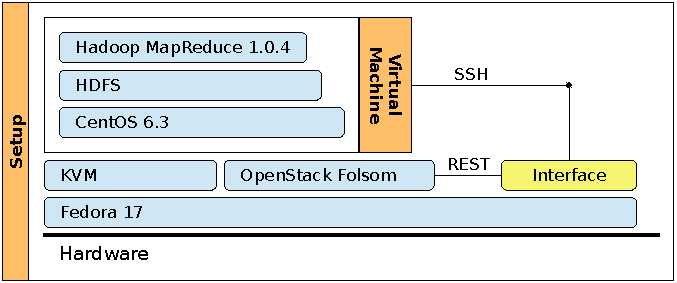
\includegraphics[width=0.85\textwidth]{imagenes/022.pdf}
 \caption{Detailed global architecture}
\label{fig:arquitecturadetalle}
\end{center}
\end{figure}

Figure \ref{fig:arquitecturainterfaz} shows the modular decomposition of qosh orchestration module.

\begin{figure}[bp]
\begin{center}
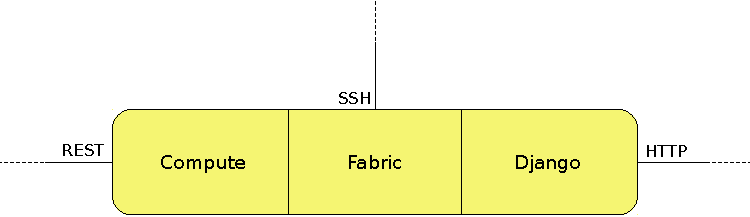
\includegraphics[width=0.8\textwidth]{imagenes/023.pdf}
 \caption{Core qosh modular decomposition}
\label{fig:arquitecturainterfaz}
\end{center}
\end{figure}

\begin{description}
 \item[Compute:] Acts as client to OpenStack REST API. It handles every interaction with the cloud decoupling qosh fromt the particular IaaS Cloud.
 \item[Django:] Is used in qosh to let users manage their MapReduce executions with ease via a web interface.
 \item[Fabric:] Is the Python library included in qosh to configure the virtual cluster deployment and destruction.
\end{description}

\subsection{Design Diagrams}\label{subsec:diagramasaltonivel}
\noindent Below are shown the design diagrams that make up the section on high level overview of the project.

\subsubsection{Django Components}\label{subsubsec:componentesdjango}
\noindent Figure \ref{fig:instalaciondjango} portrays modules adjacent to Django to support its operation.

\begin{figure}[bp]
\begin{center}
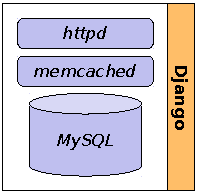
\includegraphics[width=0.23\textwidth]{imagenes/024.pdf}
 \caption{Django setup}
\label{fig:instalaciondjango}
\end{center}
\end{figure}

\begin{description}
 \item[Apache httpd:] Relied on to manage user interaction with OpenStack Dashboard, it may also be used to with qosh web interface. Initially, qosh depends on Python web server module to handle user requests, but \emph{httpd} might be easily configured.
 \item[memcached:] Is employed to cache web pages in order to speedup load times.
 \item[MySQL:] Chosen relational DBMS to store job meta-data.
\end{description}


\subsubsection{Use Cases Diagram}\label{subsubsec:casosuso}
\noindent Figure \ref{fig:casosuso} displays the set of use cases that have been considered for qosh. It reflects the five fundamental agents comprising the system.

\begin{figure}[tbp]
\begin{center}
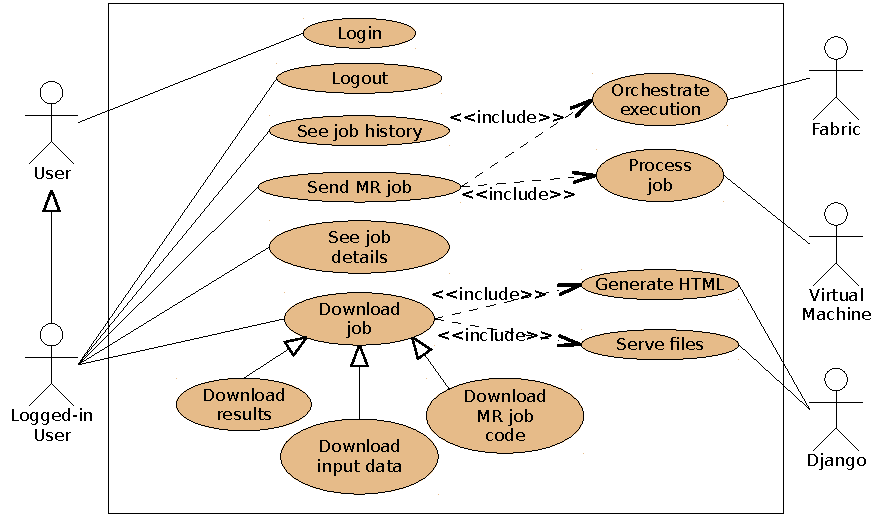
\includegraphics[width=0.99\textwidth]{imagenes/025.pdf}
 \caption{Use Cases Diagram}
\label{fig:casosuso}
\end{center}
\end{figure}

\subsubsection{Machine State Diagram}\label{subsubsec:navegacion}
\noindent Figure \ref{fig:navegacion} presents a summary on the navigation flow across the web interface. An example interaction is subsequently described.

Initially, the user is presented the \emph{Login} page so that he/she could log into qosh. If the supplied credentials were cleared --- the user must be previously registered in Keystone as user/pass is shared with qosh ---, the \emph{Main} page is shown. From there the user may \emph{Configure Job} or go over the \emph{Job History} to get some \emph{Job Details}.

\begin{figure}[tbp]
\begin{center}
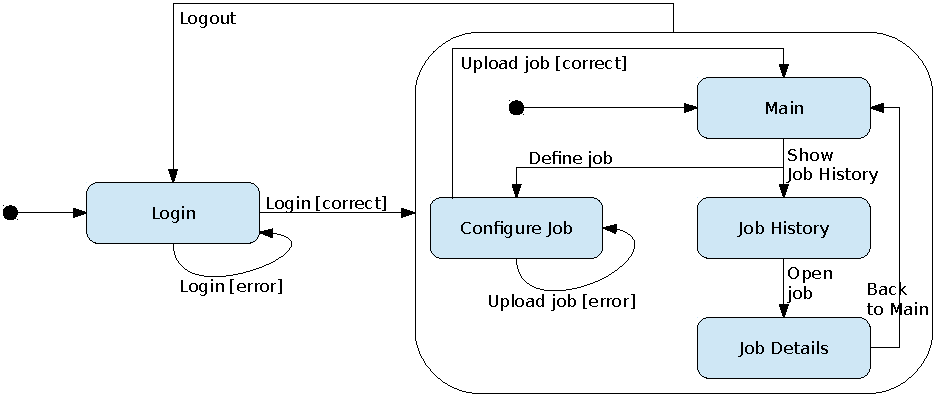
\includegraphics[width=0.99\textwidth]{imagenes/026.pdf}
 \caption{Web interface transitions}
\label{fig:navegacion}
\end{center}
\end{figure}

\subsubsection{Class Diagram --- Compute Module}\label{subsubsec:diagramaclasescompute}
\noindent Figure \ref{fig:diagramaclasescompute1} shows a small Class Diagram describing how the REST client is related to Fabric and Python.

\begin{description}
 \item[json:] Parses structured JSON-formated data and permits its manipulation. OpenStack REST API understands both XML and JSON.
 \item[Exception:] Python class representing a generic exception.
 \item[ServiceError:] Extends \texttt{Exception} to notify and handle any error that may be raised during execution. It's objects have two properties: an HTTP error code and error description.
 \item[Environment:] Contains the set of global options for configuring the virtual deployment.
 \item[httplib:] The Python module containing functions, classes and helpers toward interacting with HTTP connections. qosh banks on it to help consume the OpenStack REST service.
\end{description}

\begin{figure}[tbp]
\begin{center}
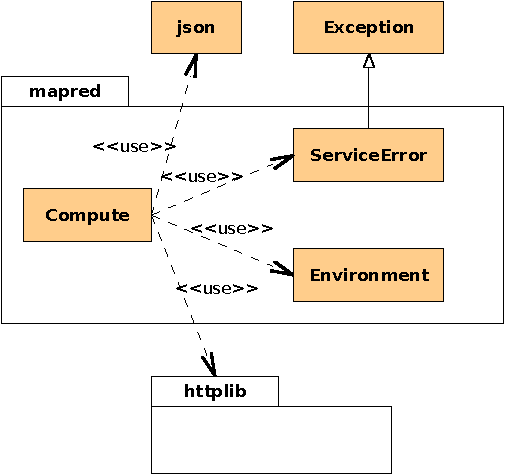
\includegraphics[width=0.5\textwidth]{imagenes/027.pdf}
 \caption{Class Diagram --- Compute module (I)}
\label{fig:diagramaclasescompute1}
\end{center}
\end{figure}

\section{Implementation}\label{sec:implementacion}
\noindent All the three modules conforming qosh core have been written in Python. The tests of the first version run over Fabric 1.4.3, Django 1.4.2 and Python 2.7.3. The configuration inside the VM is carried out by three \emph{Bash-Script}s in three different instants in the VM life cycle: before bringing the network up, after having completed the boot sequence and before shutdown. They will be detailed in section \ref{subsec:maquinavirtual}.

\subsection{Hadoop Virtual Machine}\label{subsec:maquinavirtual}
\noindent The Hadoop virtual machine is a vital asset for the qosh project; in the end it is Hadoop who executes workflows. The versions configured are Hadoop 1.0.4 and Oracle JRE 1.7. Installing and tunning every service in the VM has not been a complex process, whereas it has been long and interesting enough, for it is potentially reusable to create other customized VMs, to list every step followed to complete the setup.

\begin{itemize}
 \item In the local development machine the \emph{Virtual Machine Manager} (package \texttt{virt-manager}) was installed with \texttt{yum}. \texttt{yum} automatically installed dependent libraries like \texttt{libvirt}, the Kernel Virtual Machine hypervisor module (KVM) and a wrapper to handle it (\texttt{qemu-kvm}).
 \item Through the Virtual Machine Manager, a VM with 1 GB of RAM, 4 GB for the drive image within a \texttt{qcow2} container and both APIC and ACPI was created anew.
 \item A minimal network install of CentOS 6.3 was carried through. \emph{Basic Server} was chosen as initial package set on a single ext4 partition --- no swap partition --- without LVM.
 \item After the initial boot sequence, the distribution was put to the latest stable version available.
 \item The Oracle JRE 1.7 and Hadoop 1.0.4 were downloaded from official sources and subsequently installed on the VM.
 \item A new user (\emph{hduser}) was registered and set \emph{hadoop} as its primary group. As a result, the permission of the files related to Hadoop --- configuration files and scripts ---- were updated to allow this new user to launch and kill MapReduce jobs.
 \item \texttt{sshd} was tuned to disable superuser connections and user/pass authentication method; only ssh tunnels cleared by keypairs will be permitted.
 \item Three scripts --- similar to Ubuntu \texttt{cloud-init} scripts --- were written to \texttt{/etc/init.d/cloud-*} to customize part of the VM behavior. An important feature of them being they manage injecting the public part of the keypair used for authentication into the VM file system --- in \texttt{/home/hduser/.ssh/authorized\_keys} --- when it boots, so the owner of the private part can authenticate.
 \item The \texttt{yum groups} utility was applied to remove unused services like \emph{X-server}.
 \item From the local machine the VM was terminated and its drive image was mounted with \texttt{qemu-nbd} to remove logs and user history from the VM. Then, a 5 GB zeroed-file was created with \texttt{dd} inside the VM file system, failing, for there was not enough free space to accommodate 5 GB within a 4 GB image, while filling the remaining space up with zeros. Just after that, \texttt{qemu-img} was invoked to compress the image into a new file.
 \item Next, \texttt{fdisk} was used locally to observe the VM file system block size and initial block number of the Hadoop partition --- the only partition. By multiplying both values the partition offset was obtained, allowing for the extraction of the Hadoop partition using \texttt{qemu-nbd} offset-mounting capabilities and \texttt{dd} to dump, again, to a new file.
 \item Finally, both the \emph{initram} and the kernel image were copied out from the VM to the local file system.
\end{itemize}

\subsection{Low Level Diagrams}\label{subsec:diagramasimpl}
\noindent Next comes the diagram set that exposes those features closer to qosh implementation.

\subsubsection{Class Diagram --- Compute Module}\label{subsubsec:implementacioncompute}
\noindent Figure \ref{fig:diagramaclasescompute2} expands the \emph{Compute} module details on figure \ref{fig:diagramaclasescompute1}. Notice that types on function signatures have been borrowed from Python syntax on dictionaries and lists for brevity.

\begin{figure}[tbp]
\begin{center}
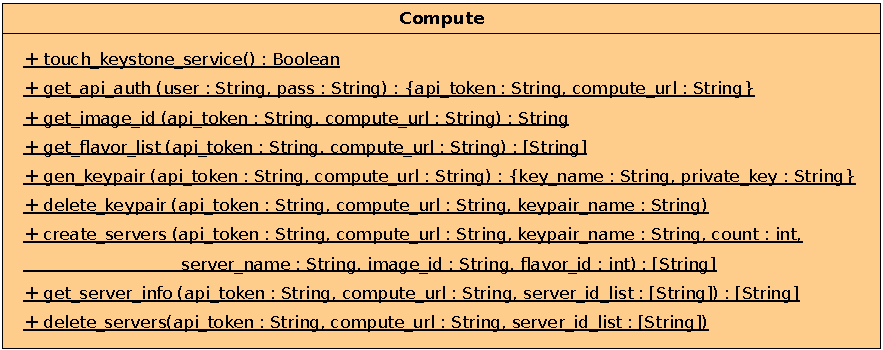
\includegraphics[width=0.99\textwidth]{imagenes/028.pdf}
 \caption{Class Diagram --- Compute module (II)}
\label{fig:diagramaclasescompute2}
\end{center}
\end{figure}

\begin{description}
 \item[List of type T:] \texttt{[T]}
 \item[Dictionary:] \texttt{\{<Key1> : <T1>, <Key2> : <T2> ... \}}
\end{description}

\subsubsection{Class Diagram --- Django and Fabric}\label{subsubsec:clasesdjangofabric}
\noindent Figure \ref{fig:djangoyfabric} exposes the relationship between the most important Django and Fabric modules.

\begin{figure}[tbp]
\begin{center}
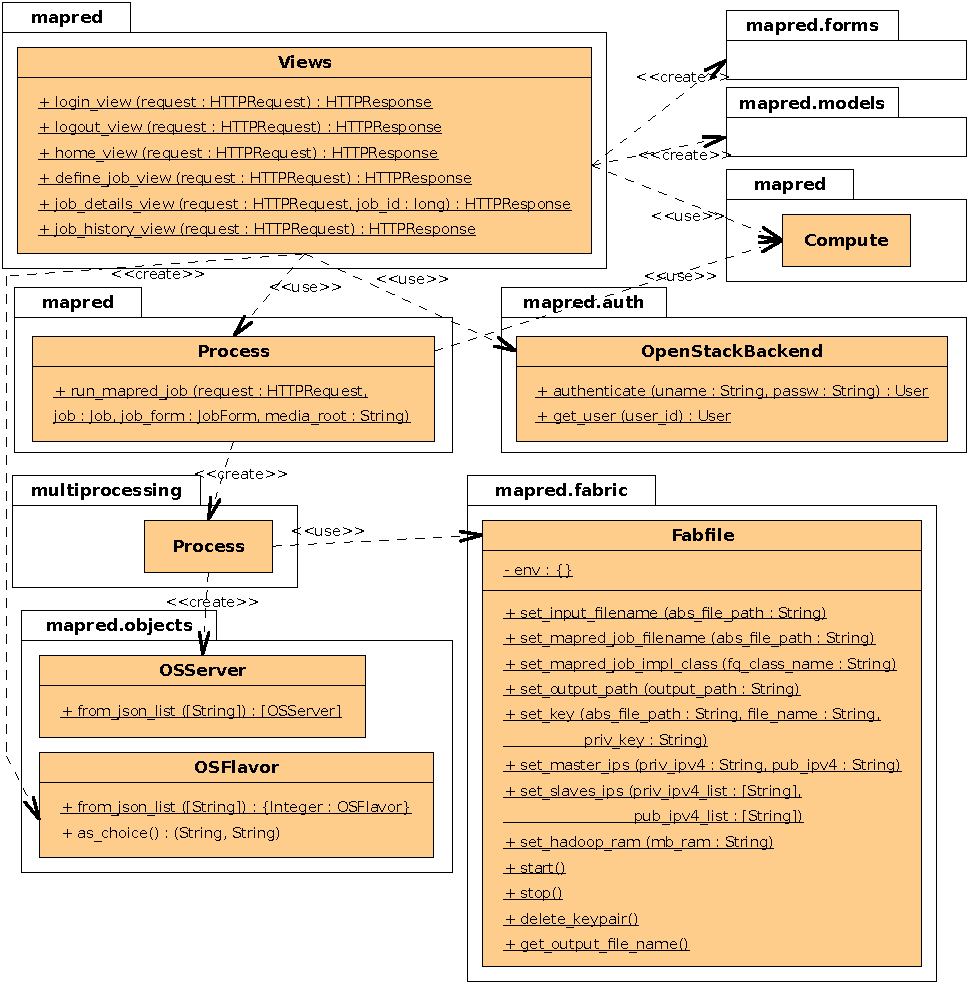
\includegraphics[width=0.99\textwidth]{imagenes/029.pdf}
 \caption{Class Diagram --- Django and Fabric}
\label{fig:djangoyfabric}
\end{center}
\end{figure}

\begin{description}
 \item[Views:] Is a delegate class implementing the behavior on each \emph{view}. It interacts with qosh Compute module to communicate with the cloud.
 \item[Process:] Is a \texttt{multiprocessing.Process} wrapper class encapsulating the logic to create processes that will handle Hadoop workflows execution collaborating with \texttt{Compute} and \texttt{Fabric} modules.
 \item[OpenStackBackend:] Is a small class that manages user logins. It is plugged into Django authenticating pipeline to delegate the clearing of user credentials to Keystone. In so doing, user access details will remain securely stored with Keystone with no need to have them duplicately stored.
 \item[OSServer y OSFlavor:] Are a kind of \emph{Transfer Object}s holding a subset of the outputted JSON data returned from the invocation of OpenStack REST API.
\end{description}

\subsubsection{Class Diagram --- Django Objects}\label{subsubsec:clasesobjetosdjango}
\noindent Figure \ref{fig:clasesobjetosdjango} details the relationships among the set of classes implementing the interaction with the web interface as provided by Django.

\begin{figure}[tbp]
\begin{center}
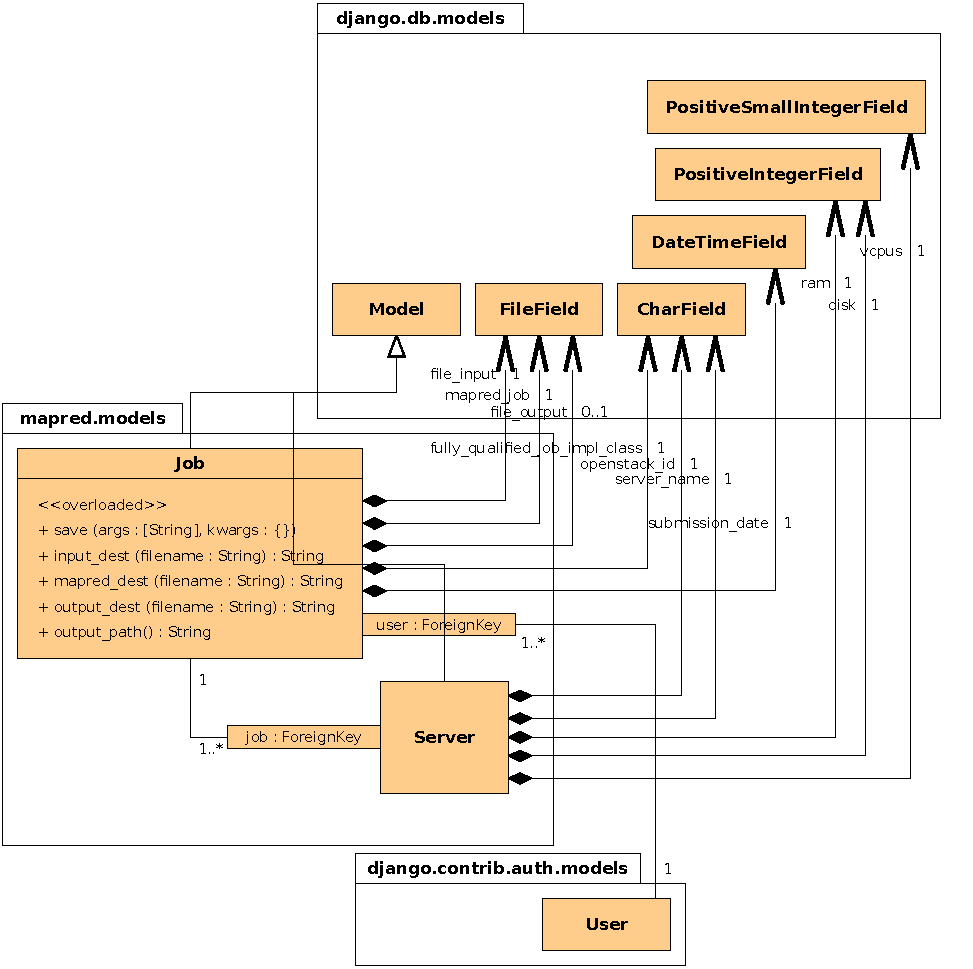
\includegraphics[width=0.99\textwidth]{imagenes/030.pdf}
 \caption{Class Diagram --- Django Objects}
\label{fig:clasesobjetosdjango}
\end{center}
\end{figure}

\begin{description}
 \item[django.db.models:] The objects defined therein model the business logic of our application. Django supplies a large set of templates that may be extended and/or composed to implement the particularities of different applications.
  \begin{description}
   \item[Model:] Is the base class of the object model supporting the business logic. Every object within the \emph{model layer} of our application extends this class --- i.e. \texttt{Job} and \texttt{Server}. Django object-relational mapper automatically translates this object model into a relational model as well as object-based queries into SQL ones.
   \item[Fields:] Hold the information related to object model classes helping Django persist the properties of the objects in a relational data base.
  \end{description}
 \item[Job:] Holds the meta-data of a Hadoop MapReduce workflow. MySQL will store these data persistently, meanwhile the file system in the Cloud Controller will actually store the information associated with the execution --- the jar file with the implementing MapReduce algorithm, inputs and outputs.
 \item[Server:] Contains the operating features of each virtual machine that had been part of a Hadoop job.
 \item[User:] Is the {Transfer Object} that is used to convey user-related information from the authorization back-end to the web interface.
\end{description}

\subsubsection{Class Diagram --- Django Forms}\label{subsubsec:clasesformulariosdjango}
\noindent Figura \ref{fig:clasesformulariosdjango} shows the class breakdown supporting the job configuration-holding forms of the web interface. \texttt{django.forms} package is laid out like the \texttt{django.db.models} package discussed above, being in this case \texttt{Form}, together with any \texttt{Field} required, the extensible class Django provides to concrete user forms.

\begin{figure}[tbp]
\begin{center}
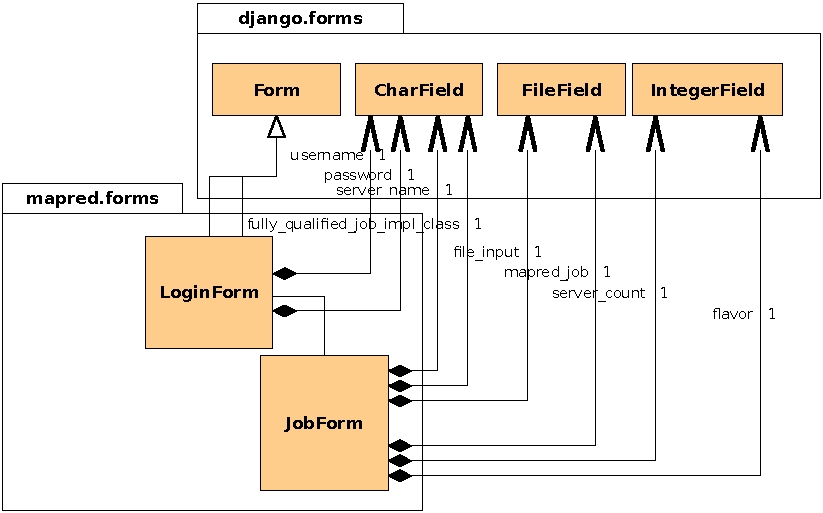
\includegraphics[width=0.99\textwidth]{imagenes/031.pdf}
 \caption{Class Diagram --- Django Forms}
\label{fig:clasesformulariosdjango}
\end{center}
\end{figure}

\begin{description}
 \item[LoginForm:] Is the user sign in form. Made up of two character fields holding the user name and password.
 \item[JobForm:] As its name suggests, is the form that allows for defining the workflow configuration. It is formed up by a set of \texttt{Fields} containing the following information: the virtual server name prefix, the qualified name of the Java class implementing the Mapper and Reducer, the input file, the \texttt{jar} package, the number of virtual servers to be deployed and their computational \emph{flavor}.
\end{description}


\subsubsection{Entity-Relationship Diagram}\label{subsubsec:entidadrelacion}
\noindent It has been pointed briefly that Django can automatically build the data base logical model derived from the object schema as written by the developer. And as expected, \emph{CRUD} operations on the DB are also managed by Django. Figure \ref{fig:entidadrelacion} shows the actual \emph{Entity-Relationship} diagram of the schema that is contained in the DB.

\begin{figure}[bp]
\begin{center}
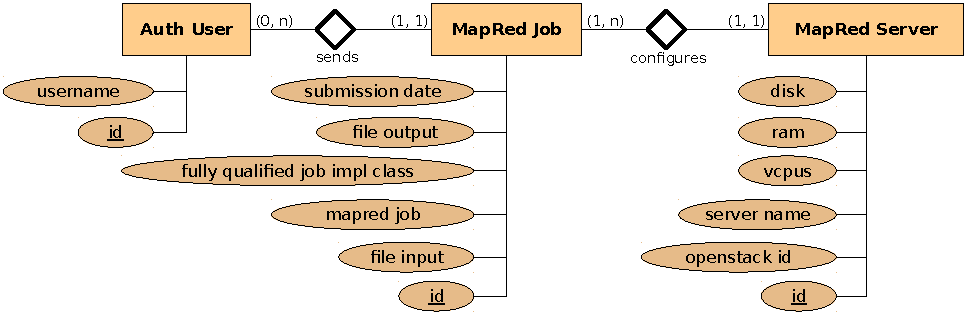
\includegraphics[width=0.99\textwidth]{imagenes/032.pdf}
 \caption{Entity-Relationship Diagram}
\label{fig:entidadrelacion}
\end{center}
\end{figure}

\subsubsection{Sequence Diagrams}\label{subsubsec:secuencia}
\noindent Figures \ref{fig:secuencia1} y \ref{fig:secuencia2} present two Sequence Diagams. They reflect the most interesting subset of messages that are interchanged between the different execution-participating entities. The sequences suppose that no errors raise during the interaction, that the user has previously signed in, that every job defining information is typed correctly and that the quota lets the deployment of the virtual cluster be carried through. Figura \ref{fig:secuencia1} pictures the full interaction. Figure \ref{fig:secuencia2} details the collaboration between classes after message \emph{\#24} in figure \ref{fig:secuencia1}.

\begin{figure}[tbp]
\begin{center}
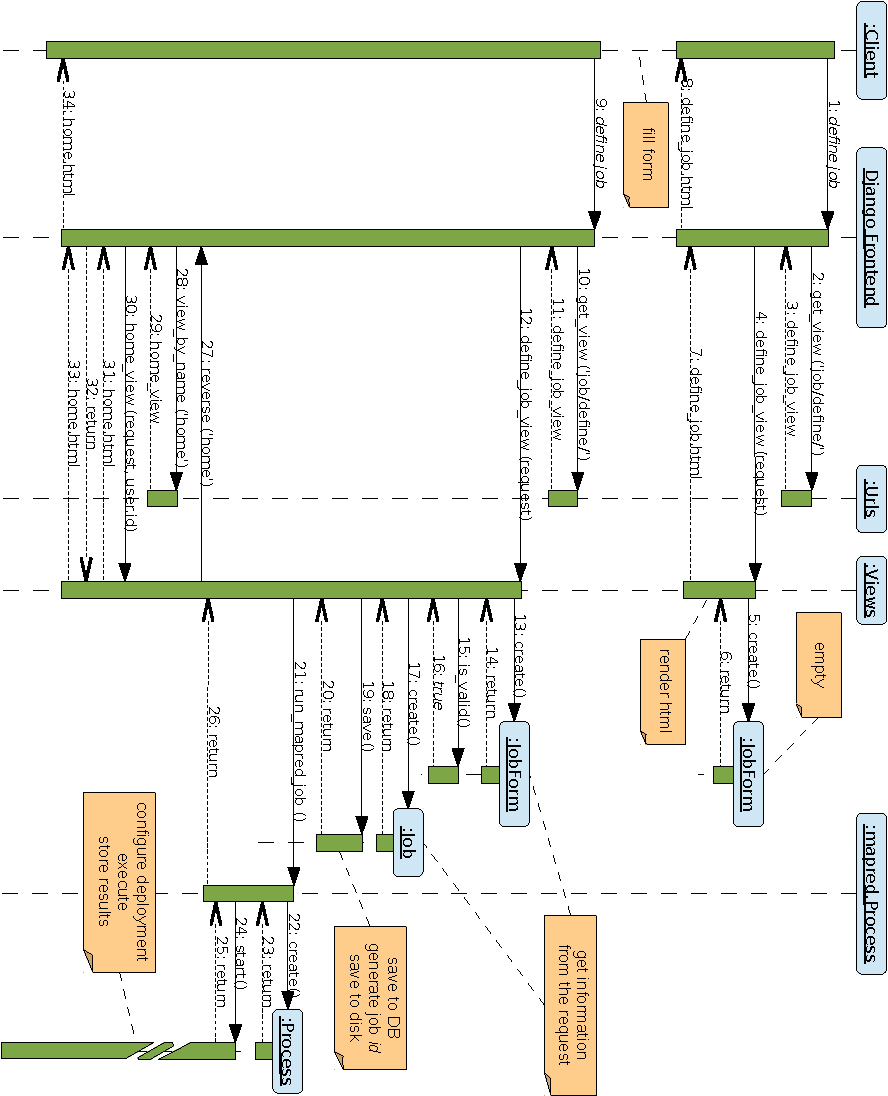
\includegraphics[width=0.99\textwidth]{imagenes/033.pdf}
 \caption{Sequence Diagram (I)}
\label{fig:secuencia1}
\end{center}
\end{figure}

\begin{figure}[tbp]
\begin{center}
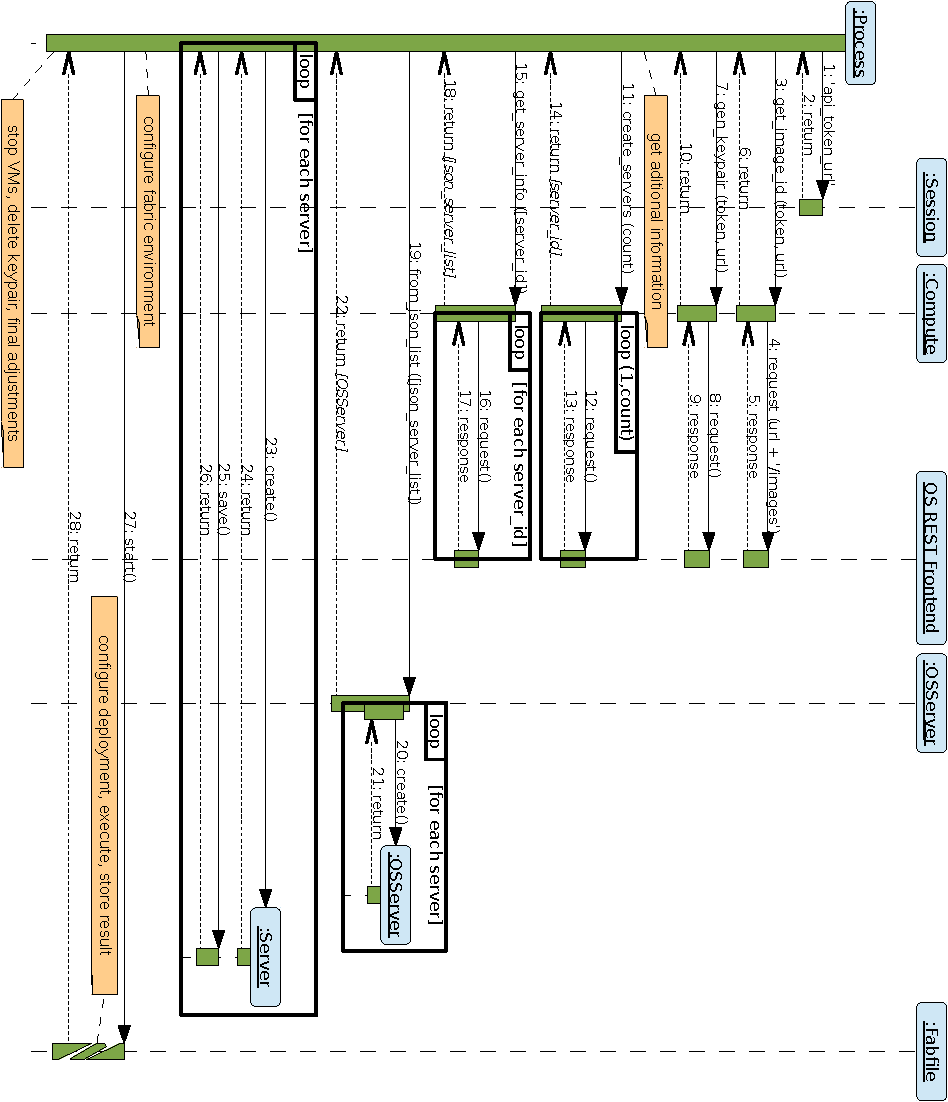
\includegraphics[width=0.99\textwidth]{imagenes/034.pdf}
 \caption{Sequence Diagram (II)}
\label{fig:secuencia2}
\end{center}
\end{figure}


%\cleardoublepage
%\chapter{Performance Analysis}\label{cap:rendimiento}
\noindent In this chapter qosh performance will be evaluated deployed over a real cluster. The execution environment will be described first and the metrics collected will be analyzed and put in context thereafter.

\section{Testing Environment}\label{sec:entornodeprueba}
\noindent Figure \ref{fig:clusterdespliegue} shows how the cluster is configured. The leftmost part of the figure shows the Cloud Controller; the rightmost, the Cloud Node. The Cloud Controller has been put through a full OpenStack Folsom installation --- except for Cinder, Swift or Quantum as they will not used ---, plus MySQL, Fabric and Qpid as message broker. In the Cloud Node only the bare minimum to support VM execution has been installed --- OpenStack Compute. The other required \emph{amenities} of the Cloud Node are delegated to the Controller via Qpid.

\begin{figure}[tbp]
\begin{center}
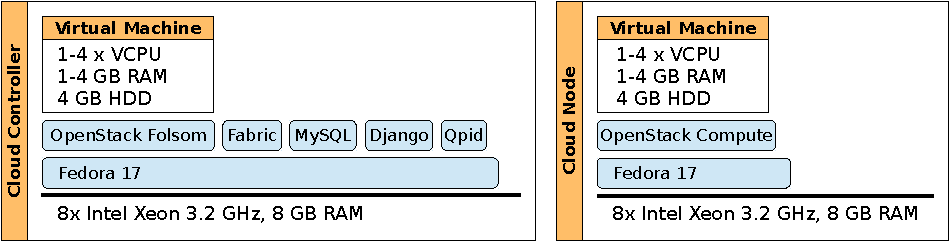
\includegraphics[width=0.99\textwidth]{imagenes/038.pdf}
 \caption{Deployment morphology}
\label{fig:clusterdespliegue}
\end{center}
\end{figure}

Regarding the physical layer, both nodes posses the same hardware configuration: Octa core Intel Xeon processor @ 3.2 \emph{GHz} with VT-x, 8 GB of RAM, 200 GB SATA 3 Gb/s 7200 RPM and Gigabit networking interface.

The Hadoop virtual image, whose creation procedure is described in section \ref{subsec:maquinavirtual}, will be used to create the VM instances that will effectively carry out the computations. Hadoop version is 1.0.4 and JRE's is 1.7v6 from Oracle. Figure \ref{fig:clusterdespliegue} shows the Hadoop VM in context. This instance will be increasingly provided from 1 to 4 GB of RAM and the same number of VCPUs to assess qosh's scaling. This varying amount of RAM will be shared between the guest OS and the JVM. The deployment has been configured to allow Hadoop to address all the memory in the VM --- except for those addresses in use by the OS and the JVM.

\section{Testing Methodology}\label{sec:metodologiaprueba}
\noindent This section contains both in and out scalability analysis and a study on the behavior on increasing input sizes. To evaluate how qosh scales, a map reduce work flow, large enough to stress every instance in the virtual cluster, will be fed to Hadoop; the work flow will count the words in 62.5 MB of plain text.

To actually assess the horizontal scalability, the size of the virtual cluster will progressively be doubled starting from one instance up to four. To test vertical scalability, two VMs will be initially spawned with 1 GB of RAM each, to have their RAM and VCPU count doubled on each test case until reaching 4 GB. Finally, to evaluate running time tendency input text size will be doubled from the original 62.5 MB to 250 MB.

As Glance and Compute cooperate to cache images, the time required to start an instance of some image will be longer the first time it launches, effectively skewing results. To get rid of those divergences, the instances on each flavor will be \textbf{warmed} by starting and destroying them before taking measures.

\emph{A priori}, the expected variance of the timings between executions is small enough to consider \emph{ten} to be a representative number of repeated measures --- this hypothesis will be validated \emph{a posteriori} on analyzing the results. To measure timings, the code will include a set of time marks that will help take apart the following times:

\begin{description}
    \item[Deploying:] time elapsed since the virtual cluster creation request is send until every instance is accessible.
    \item[Configuring:] time required to establish the Hadoop execution environment. It comprises the time to configure the virtual Hadoop cluster plus the time to distribute input data onto HDFS.
    \item[MapReducing:] time dedicated by Hadoop to execute the \emph{wordcount} work flow.
    \item[Cleaning:] time required to wipe out the execution environment. It does not include the time it takes OpenStack to completely remove the instances.
    \item[Total:] 
\end{description}

It should be noted that the timings shown are the averaged results of the ten executions in each case.

\section{Analysis of the Results}\label{sec:analisisresultados}

\begin{figure}[tbp]
\begin{center}
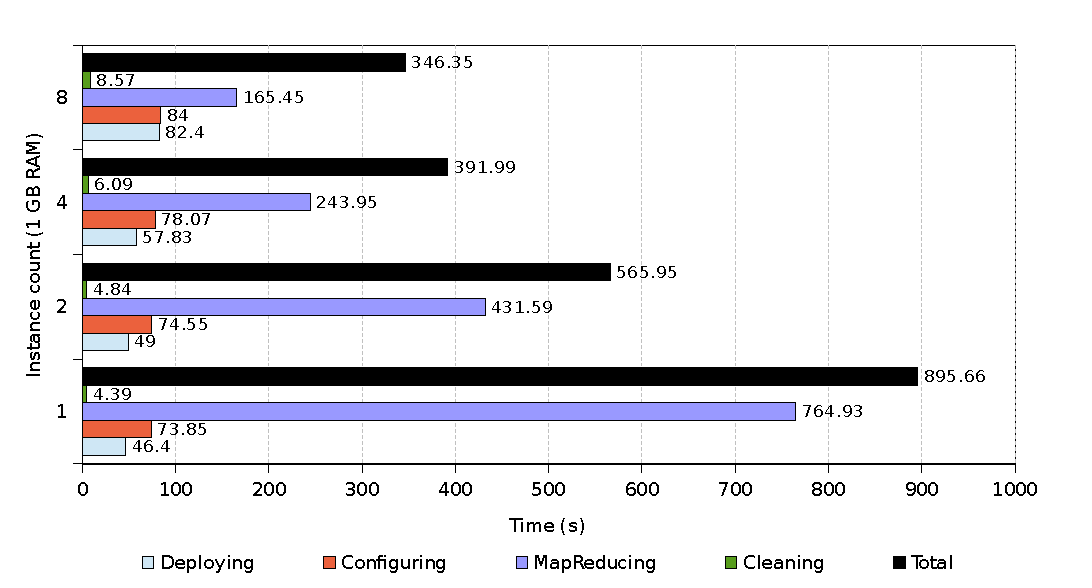
\includegraphics[width=0.98\textwidth]{imagenes/039.pdf}
\caption{Scaling out}
\label{fig:eschorizontal}
\end{center}
\end{figure}

\noindent Figure \ref{fig:eschorizontal} shows the evolution of the different timings as the instance count increases from one to eight. It may be observed that deployment, configuring and cleaning time raise with the number of instances deployed, meanwhile processing time is reduced. I.e, the time required for a virtual cluster to deploy, configure and delete every instance depends only on its size --- as it could have been hypothesized. On the other hand, MapReducing time --- and thus total time --- is also bound to input size. Figure \ref{fig:escvertical} presents the tendency of the five timings as the cluster is scaled in from 1 GB of VCPU and RAM to 4 each.

\begin{figure}[tbp]
\begin{center}
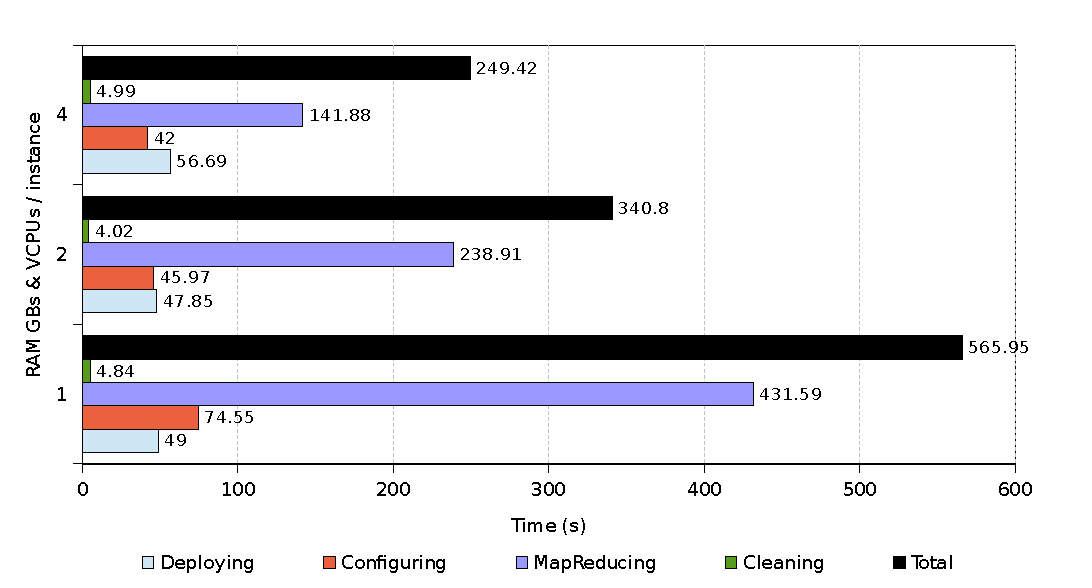
\includegraphics[width=0.98\textwidth]{imagenes/041.pdf}
\caption{Scaling in}
\label{fig:escvertical}
\end{center}
\end{figure}



A la vista de esta figura, tal vez lo m\'as llamativo sean los tiempos de des\-plie\-gue y borrado, pudiendo considerarse pr\'acticamente constantes a pesar de aumentar la capacidad de c\'alculo de las instancias. Dicho de otro modo, la dificultad que supone desplegar o borrar un cl\'uster virtual en nuestro entorno depende exclusivamente del n\'umero de instancias o nodos virtuales ---conclusi\'on que ya hab\'iamos alcanzado previamente. Precisamente, hab\'iamos observado c\'omo la complejidad de configuraci\'on crec\'ia proporcionalmente con el tama\~no del cl\'uster. En este caso sucede lo contrario: al estar mejorando las caracter\'isticas t\'ecnicas de las dos instancias, los tiempos de configuraci\'on de Hadoop se ven l\'ogicamente reducidos. Es decir, la conclusi\'on revisada dicta que el tiempo de configuraci\'on var\'ia de forma directa con el n\'umero de instancias y de forma inversa con las capacidades operativas de las mismas. \newline

Los resultados contenidos en estas gr\'aficas demuestran que nuestra soluci\'on se comporta de modo m\'as eficaz cuando se mejora la capacidad de c\'omputo de las instancias ---escalabilidad vertical--- en vez de aumentar el tama\~no del cl\'uster virtual soporte ---escalabilidad horizontal. Este hecho se observa con claridad en las figuras \ref{fig:eschorizontal} y \ref{fig:escvertical} al comparar los casos extremos de prueba: ocho instancias de 1 GB de RAM frente a 4 GB de RAM y VCPUs por ins\-tan\-cia, respectivamente. Ambos casos distribuyen sendos clusters virtuales con las mismas caracter\'isticas de 8 VCPUs y 8 GB de RAM sobre nuestros nodos de prueba. Sin embargo, el tiempo de ejecuci\'on total es casi un \texttt{28\%} menor al mejorar las dos instancias (figura \ref{fig:escvertical}); esperable, en cierta medida, al ahorrar la sobrecarga de comunicaci\'on por la red. \newline

\begin{figure}[tbp]
\begin{center}
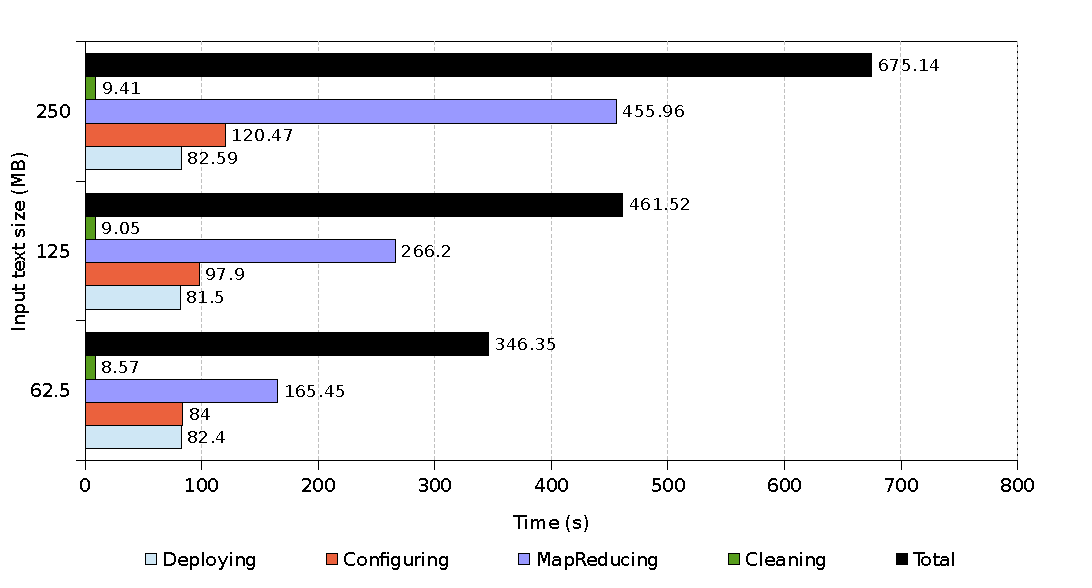
\includegraphics[width=0.98\textwidth]{imagenes/042.pdf}
\caption{Tama\~no de entrada frente a tiempo de ejecuci\'on}
\label{fig:evotemporal}
\end{center}
\end{figure}

La figura \ref{fig:evotemporal} muestra la evoluci\'on de los tiempos de ejecuci\'on al incrementar la magnitud de los datos a procesar. Como era de esperar, la duraci\'on de la etapa MapReduce y la duraci\'on total crecen en relaci\'on directa con el tama\~no de entrada, pero en menor medida. Los tiempos de despliegue y bo\-rra\-do se mantienen pr\'acticamente constantes en cada caso, mientras que el tiempo de configuraci\'on crece ligeramente, al englobar la descompresi\'on y posterior distribuci\'on de los ficheros de entrada sobre el cl\'uster Hadoop.

%\cleardoublepage
%\chapter{Trabajo relacionado}\label{cap:conclusiones}
\noindent The present chapter describes other particular solutions for executing MapReduce applications. Each one's characteristics will be briefly explored by contrasting them against qosh's.

\section{Amazon Elastic MapReduce}\label{sec:emc}
\noindent \emph{Amazon Elastic MapReduce} \cite{aws} exposes a web service interface that allows the user to send MapReduce execution requests. EMR is supported internally by Amazon EC2 to provision, on demand, the required infrastructure by the MapReduce work flow. Thus, an EMR user will not have to worry about provisioning, creating, configuring and destroying the virtual clusters that would support execution. This convenient transparency to the user comes with a series of important limitations:

\begin{description}
    \item[Underlying infrastructure restriction]: being as it is a service owned by Amazon, it was expected that usage of computational resources out of their reach were limited; and so it is: EMR users will not be able to couple their virtual instances to other clouds that may incur in lower exploitation costs.
    qosh, as it has been shown, separates and exposes responsibilities in a way that using a different cloud, for example, requires only adapting a new Compute module to the particular REST API of the cloud that would be used.
    \item[Installation restriction]: it is not possible to deploy a custom-built VM to execute MapReduce applications in EMR. qosh will handle work flows driving a Hadoop VM with a loose coupling with the deploying subsystem (Fabric) with a doble end:
    \begin{itemize}
        \item To ease VM customizations and upgrades (Kernel, Hadoop, JRE, etc.).
        \item To give the possibility to create custom VMs from scratch.
    \end{itemize}
    \item[Information restriction:] some users are under non disclosure agreements that render impossible sharing data with third parties like Amazon, effectively leaving those services out of the equation. qosh's open source nature makes it easy for a developer to adapt qosh to its concrete functional requirements with no sharing of private data.
\end{description}

EMR node typology is described next. EMR clusters present three kinds of nodes:

\begin{description}
    \item[Master:] this node, unique per EMR cluster, executes both a NameNode and a JobTracker.
    \item[Core:] this kind of nodes store data and process job tasks. The are basically comprised of a DataNode and a TaskTracker.
    \item[Task:] they only run TaskTracker processes.
\end{description}

qosh deploys clusters with a single hybrid master-worker node --- with NameNode, JobTracker, DataNode and TaskTracker --- being the rest worker nodes --- with DataNode and TaskTracker only. This deployment configuration could be easily altered to fit into diverse use cases by rewriting the \texttt{mapred.fabric.fabfile} module.

Regarding the execution flow, EMR allows for keeping the instances alive when they had finished scheduled processing to avoid the computational overhead of their spawning. qosh's default behavior is to destroy instances upon completion. As expected, defaults may be easily overridden.

EMR draws on Amazon S3 to store input data to Hadoop as well as to write final results. Intermediate information is stored within the virtual instances and is destroyed as they are. qosh uses the file system of the Controller Node to store I/O data from the virtual cluster, and, like EMR, employs the virtual instances' file system to save intermediate data. qosh may also be plugged a different repository to store final results. To that end, a new back end module would have to be written for Django to correctly locate data and update the DB to point elsewhere.

\section{Resilin}\label{sec:resilin}
\noindent \emph{Resilin} \cite{resilin} main intention is to improve EMR by trying to overcome its limitations. The development team has written an API (see figure \ref{fig:arquitecturaresilin}) capable of receiving EMR-like requests that will translate into two kinds of actions:

\begin{itemize}
    \item An interaction flow with an IaaS Cloud to create and destroy instances (what qosh does in its Compute module).
    \item An SSH connection to the virtual Hadoop cluster to configure and execute tasks (what qosh does with its Fabric module).
\end{itemize}

\begin{figure}[tbp]
\begin{center}
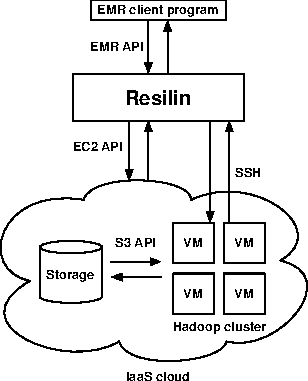
\includegraphics[width=0.5\textwidth]{imagenes/035.pdf}
 \caption{Resilin architecture. Source: \cite{resilin}}
\label{fig:arquitecturaresilin}
\end{center}
\end{figure}

Information storage and I/O is delegated upon an S3 compatibility adaptor supported both by Nimbus and Eucalyptus --- with \emph{Cumulus} and \emph{Walrus} respectively.

Besides, and maybe the most interesting Resilin trait, its implementors experiment with the possibility to execute MapRecude work flows atop infrastructure provided by different clouds. Though it may not be the general approach to provision private infrastructure to virtual deployments due to the inherent heterogeneity among different IaaS frameworks, it might prove useful when the infrastructure has to be drawn upon from public clouds. In the abstract, the idea has been implemented bridging deployments on different clouds by exposing instances on one cloud to the other cloud Master Node as if they were part of the same virtual cluster.

qosh does not support hybrid cloud deployments. Yet, it cloud be implemented without much ado modifying the Compute module accordingly.

The bottom line is that Resilin is the solution resembling qosh the most; delegating the reduction of MapReduce work flows on Hadoop and the virtual deployments on an IaaS Cloud EC2-compatible --- all of the four evaluated in \ref{sec:frameworksevaluados} are. Lastly, figure \ref{fig:resilinproyecto} lists the different tools that aid supporting the functionality exposed.

\begin{figure}[tbp]
\begin{center}
\begin{tabular}{|c|c|c|}
\hline
& \textbf{Resilin} & \textbf{qosh} \\
\hline
\textbf{Global} & \texttt{Python} & \texttt{Python} \\
\hline
\textbf{HTTP} & \texttt{Twisted} & \texttt{Django} \\
\hline
\textbf{IaaS Cloud interaction} & \texttt{boto} & \texttt{Compute} (custom module) \\
\hline
\textbf{Virtual instances interaction} & \texttt{paramiko} & \texttt{Fabric} \\
\hline
\end{tabular}
\caption{Tool listing}
\label{fig:resilinproyecto}
\end{center}
\end{figure}

\section{Cloud MapReduce}\label{sec:cloudmapred}
\noindent \emph{Cloud MapReduce} representa una aproximaci\'on diametralmente opuesta a Resilin. Mientras Resilin pretende implementar un API MapReduce centr\'andose en \emph{organizar} los distintos componentes necesarios, Cloud MapReduce se apoya en los servicios de un cloud ---en concreto el de Amazon--- para implementar el modelo MapReduce \cite{googlemapreduce} \emph{directamente} sobre \'el.\newline

A continuaci\'on comentamos algunas propiedades de Cloud MapReduce que consideramos m\'as relevantes:

\begin{description}
\item[Escalabilidad incremental:] es la capacidad de a\~nadir nuevos nodos al cl\'uster MapReduce cuando el trabajo ya ha comenzado; de tal forma que las nuevas instancias se informen autom\'aticamente del estado global del trabajo y se asignen tareas ellas mismas. Resilin \cite{resilin} lo soporta tambi\'en, nuestro proyecto no.
\item[Simetr\'ia y descentralizaci\'on:] con esta idea se pone manifiesto la falta de jerarqu\'ia en los despligues: cada nodo de un cl\'uster tendr\'a las mismas responsabilidades que sus colegas. Este representa el primer punto de distinci\'on importante frente a las dem\'as aproximaciones ---MapReduce, Hadoop, Amazon EMR, Resilin y nuestro proyecto--- en las que la configuraci\'on, reparto, planificaci\'on, etc. de los trabajos y tareas tiene lugar dentro de los nodos maestro, y la ejecuci\'on y almacenamiento sucede en los esclavos. En Cloud MapReduce los nodos act\'uan de modo independiente, controlando el estado global del trabajo para determinar qu\'e tarea se adec\'ua mejor a las necesidades instant\'aneas del flujo de trabajo. Se debe citar asimismo, que esta simetr\'ia de Cloud MapReduce hace que sea menos problem\'atico superar los problemas en los maestros.
\item[Heterogeneidad:] entendida con una doble componente: por una parte, la posible coexistencia de instancias de distintos \emph{sabores} ---siguiendo la notaci\'on de Amazon--- en un mismo trabajo, y por la otra, la capacidad de crear instancias en m\'ultiples clouds. Resilin soporta ambas cuestiones, nuestra propuesta no.
\end{description}

En Cloud MapReduce el almacenamiento global ---la E/S y los datos intermedios--- se hace sobre S3, la comunicaci\'on y sincronizaci\'on entre nodos con el servicio de colas de Amazon (\emph{SQS} o \emph{Simple Queue Service}) y el almacenamiento de estado de las tareas y nodos en el servicio de base de datos de Amazon, \emph{SimpleDB}. En nuestro proyecto, el almacenamiento global se hace sobre el sistema de ficheros del servidor web; que probablemente no sea la mejor opci\'on debido a las limitaciones de ancho de banda y la falta de tolerancia a fallo. Para modificar este comportamiento, ser\'ia necesario, por ejemplo, dise\~nar un backend de datos personalizado y acoplarlo al \emph{pipe} de almacenamiento de Django, o montar alg\'un sistema de ficheros y apuntar a Django en su direcci\'on. En cuanto a la sincronizaci\'on, comunicaci\'on y estado de las instancias, se delega toda esa funcionalidad en Hadoop.\newline

Por \'ultimo se presenta la figura \ref{fig:arquitecturacloudmapreduce}, que recoge la instant\'anea de alto nivel de un instante de la ejecuci\'on de un trabajo en el Cloud MapReduce. Esta figura recuerda, y no casualmente, a la figura \ref{fig:exmapreduce} que presentaba las fases t\'ipicas de procesamiento del paradigma MapReduce original \cite{googlemapreduce}.

\begin{figure}[tbp]
\begin{center}
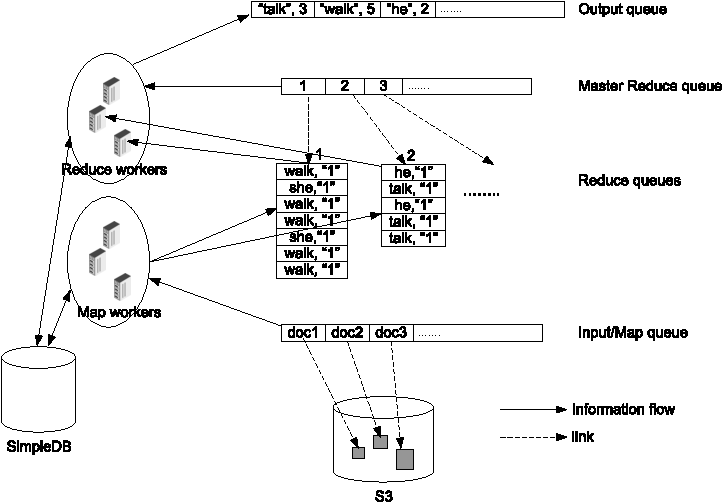
\includegraphics[width=0.9\textwidth]{imagenes/036.pdf}
 \caption{Arquitectura de Cloud MapReduce. Fuente: \cite{cloudmapreduce}}
\label{fig:arquitecturacloudmapreduce}
\end{center}
\end{figure}

\section{Dynamic Cloud MapReduce}\label{sec:dynamicmapreduce}
\hyphenation{SmartFrog}
\noindent La figura \ref{fig:arquitecturadynamicmapreduce} presenta la arquitectura de la soluci\'on propuesta en \cite{dynamicmapreduce} para la apropiaci\'on y configuraci\'on autom\'aticas de infraestructura virtual que procesar\'a aplicaciones MapReduce. Como se ve, los componentes de alto nivel se corresponden directamente con los de nuestra aproximaci\'on; sin embargo (\emph{Dynamic Cloud MapReduce}) presenta algunas diferencias.

\begin{figure}[tbp]
\begin{center}
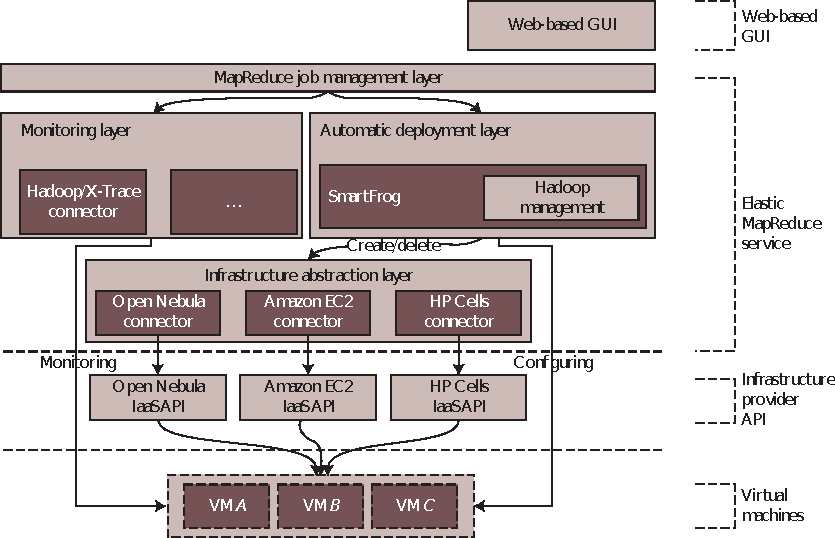
\includegraphics[width=0.9\textwidth]{imagenes/037.pdf}
 \caption{Dynamic Cloud MapReduce. Fuente: \cite{dynamicmapreduce}}
\label{fig:arquitecturadynamicmapreduce}
\end{center}
\end{figure}

\begin{description}
\item[GUI:] a pesar de que la interfaz con el usuario tambi\'en es una p\'agina web, en este caso han implementado un servicio \emph{RESTful} (la capa de direcci\'on de los trabajos MapReduce) que desacopla el manejo del servicio de procesamiento MapReduce. Adem\'as, dicha capa permite que los usuarios del despliegue encadenen la ejecuci\'on de m\'ultiples trabajos MapReduce. En nuestra propuesta hemos implementado las acciones de despliegue y procesado formando parte de la mec\'anica de la web. Este \'ultimo punto, el encadenamiento de flujos MapReduce, no se soporta.
\item[Monitoring Layer:] como su nombre indica, es una capa orientada a la monitorizaci\'on de los procesos MapReduce. Si bien no hemos integrado esta caracter\'istica en la interfaz web, tampoco hemos limitado el acceso a los servicios de monitorizaci\'on integrados en Hadoop; en referencia a los comentados microservidores web de cada m\'odulo \emph{Tracker}.
\item[Automatic Deployment Layer:] con esta capa software se controla el des\-plie\-gue virtual. Equivale a nuestro m\'odulo \emph{Fabric} (\texttt{fabfile.py}). La diferencia fundamental, a parte de que usan \emph{SmartFrog} para gestionar el despliegue, es que la m\'aquina virtual parte de una instalaci\'on \emph{limpia} del sistema operativo a la que se le ha agregado exclusivamente  SmartFrog. De manera que, antes de ejecutar cada flujo MapReduce, SmartFrog gestiona la descarga, instalaci\'on y configuraci\'on de Hadoop en cada m\'aquina virtual. Esta aproximaci\'on es m\'as flexible que la propuesta en el proyecto ---nos apoyamos en una imagen con Hadoop y el JRE preinstalados---, pero a\~nade una importante sobrecarga de descarga y configuraci\'on.
\item[Infrastructure Provider Abstraction Layer:] con esta fachada separan la sintaxis del servicio REST del cloud concreto desplegado, permitiendo definir adaptadores para cada uno. En nuestra propuesta no hemos aislado una interfaz que permita definir adaptadores de forma transparente. Sin embargo, y tal como se ha apuntado, bastar\'ia definir el comportamiento de las funciones del m\'odulo \texttt{Compute} (\texttt{compute.py}) y adaptar los \emph{Transfer Objects} (\texttt{objects.py}) a cada sintaxis.
\end{description}

Por \'ultimo, hacer constar que la opci\'on elegida para el almacenamiento es muy parecida a la propuesta ---\emph{HDFS} y sistema de ficheros local. Sin embargo, nuestra soluci\'on es autom\'atica: no requiere que el usuario suba manualmente los ficheros de entrada. Los ficheros de salida se almacenan en un servidor local y son accesibles desde la interfaz REST. En nuestra propuesta se permite que cada usuario descargue los resultados de sus procesamientos desde la interfaz web.

\section{Resumen}\label{sec:resumenconclusiones}
\noindent Teniendo en cuenta lo expuesto hasta este punto, se podr\'ia pensar que nuestra implementaci\'on es la m\'as limitada. Sin embargo, presenta una importante ventaja frente a todas las dem\'as solucciones: la \emph{absoluta simplicidad}. Lo que parece un car\'acter secundario se convierte en algo fundamental si el usuario es inexperto o si se pretende hacer un despliegue r\'apido de tecnolog\'ia MapReduce el\'astica.\newline

Ninguna de las soluciones estudiadas presenta una aproximaci\'on tan simple e integrada de instalaci\'on, configuraci\'on y explotaci\'on de infraestructura. Todas conllevan alg\'un esfuerzo adicional del usuario, requiriendo, en general: el conocimiento de su mec\'anica interna, el despliegue previo de un cloud, el abono bajo consumo o el hacer p\'ublicos los datos de entrada al framework MapReduce. En resumen, nuestro proyecto es la elecci\'on natural para des\-plie\-gues reducidos inicialmente o como punto introductorio a las tecnolog\'ias cloud IaaS y MapReduce. Partiendo de un despligue m\'inimo y autom\'atico, el administrador del cloud podr\'a agregar nuevos nodos de procesamiento, ac\-tua\-li\-zar la m\'aquina virtual Hadoop, alterar la mec\'anica de aprovisionamiento o, incluso, instalar un cloud de otro proveedor, sin demasiado esfuerzo.

%\cleardoublepage
%\chapter*{Conclusion}\label{cap:aportaciones}
\markboth{Conclusion}{Conclusion}
\addcontentsline{toc}{chapter}{Conclusion}
\noindent This section discusses a series of qosh's contributions and possible lines of development for the future.

\section*{Main Contributions}\label{sec:bondadesdeficiencias}
\noindent qosh has been designed and implemented to be the solution that will considerably reduce the complexity and cost inherent to elastic MapReduce computations. qosh automatically configures a minimum OpenStack Folsom installation before being able to drive a virtual Hadoop cluster deployed atop. As a convenient feature, qosh is also accompanied with a web interface to setup MapReduce jobs and fetch results as they finish execution.

The main qosh characteristics may be summarized as follows.

\begin{description}
    \item[Simplicity] both for installation and exploitation. The installer cannot be any easier and the web interface provides the means to define Hadoop clusters indeterminately large, send in MapReduce workflows and retrieve results directly and intuitively. The Annex \ref{cap:guiainstalacion} details a quick guide to complete a testing deployment.
    \item[Vertical integration] of every component that allows qosh function. The installation script sets up the execution environment for every level --- web, MapReduce and infrastructure --- needing no interaction from the user.
    \item[High performance] in the initial deployment. qosh has been devised to be simple and flexible but also performing. Other simple solutions like \emph{DevStack}, while easy to configure and run, impose a serious penalty to performance rendering them unable to provide the required environment to develop applications on top of OpenStack --- which, of course, it is not DevStack's main purpose.
    \item[Reusability] of fundamental components. By having followed AWS' guidelines of letting the injected meta-data configure the instances when booting, it allows any IaaS Cloud to be used --- provided it be AWS-compatible ---, or seen from another perspective, it allows the default Hadoop VM to be installed directly on a real cluster, i.e. without virtualization.
    \item[Adaptability] of qosh's to handle infrastructure from other clouds. Using the Compute module as starting point, a partial rewrite would suffice to support any IaaS Cloud.
    \item[Transparency] of the whole. The code of any module may be openly accessed, downloaded and modified --- some restrictions may apply ---; including OpenStack, Django, Fabric, Hadoop, Python and qosh.
\end{description}

\section*{Future Development}\label{sec:directricesfuturo}
\noindent One of qosh's weak points lies in the coupling among the main modules. It would be interesting to abstract an interface with the cloud's REST API access client, so that different delegates could implement it and adapt the messages to the particular cloud syntax, opening indirectly the possibility to hybrid cloud deployments.

Following those dynamics, some use cases like \emph{Show History} or \emph{Send Job}, could become objects, decouple from the web interface and be executed in an action processor object. Having unlinked those actions off the interface, it would not be hard to implement a particular REST API that would allow clients of any nature to execute MapReduce workflows. This action processor object might be designed as a thread pool that would consume object-actions fed from the interface controller, facilitating scaling out and load balancing.

%\renewcommand\chaptername{Apendice}
%\appendix
%\chapter{Installation and Exploitation --- quick-openstacked-hadoop}\label{cap:guiainstalacion}
\noindent To make a quick deployment in a single node and be able to run MapReduce work flows effortlessly, a \emph{git} repository has been set up with source files, configuration scripts, and the Hadoop VM. This guide will describe the steps required to achieve a basic installation.

\section{Quick Installation}\label{sec:instalacionqosh}

\subsection{System Requirements}\label{subsec:reqsis}
\noindent qosh's operating requirements:

\begin{itemize}
    \item x86\_64 CPU with virtualization extensions (VT-x or AMD-V).
    \item 4 GB of RAM or more.
    \item 10 GB of HDD space.
    \item Fedora 17 installation.
\end{itemize}

The amount of RAM and HDD will limit the number of concurrent instances that are allowed to run --- recall that each instance will be provisioned 1 GB of RAM and 4 GB of HDD on boot from the host computer.

\subsection{Installation}\label{subsec:instalacion}
\noindent Figure \ref{fig:comandosshel} contains the command list that will have to be typed in a terminal to run the installation and configuration scripts.

\begin{figure}[tbp]
 \begin{center}
  \begin{tabular}{|l|}
   \hline
   \texttt{{\bf \$} sudo yum install -y git} \\
   \texttt{{\bf \$} sudo yum update -y} \\
   \texttt{{\bf \$} sudo reboot} \\ \\
   \texttt{{\bf \$} cd <destination\_folder>} \\
   \texttt{{\bf \$} git clone https://code.google.com/p/quick-openstacked-hadoop} \\
   (quick-openstacked-hadoop folder will be created) \\ \\
   \texttt{{\bf \$} cd quick-openstacked-hadoop} \\
   \texttt{{\bf \$} sudo python install.py} \\
   (OpenStack Folsom, Hadoop VM, Fabric and Django will be installed) \\ \\
   \texttt{{\bf \$} python configure.py} \\
   (Django will be adjusted) \\
   \hline
  \end{tabular}
  \caption{Command sequence I}
  \label{fig:comandosshell}
 \end{center}
\end{figure}

\subsection{Test-Driving the Instalaci\'on}\label{subsec:testejecucion}
\noindent If the commands in the previous section have succeeded, OpenStack and Django should be correctly installed. To assert this, open \url{http://localhost/dashboard} in a web browser. After a few seconds there should appear the welcoming Horizon splash screen that would allow to log into OpenStack --- user name and password default to \emph{udc}. Once logged in, a web page like the one in figure \ref{fig:homeos} should be displayed.

\begin{figure}[tbp]
\begin{center}
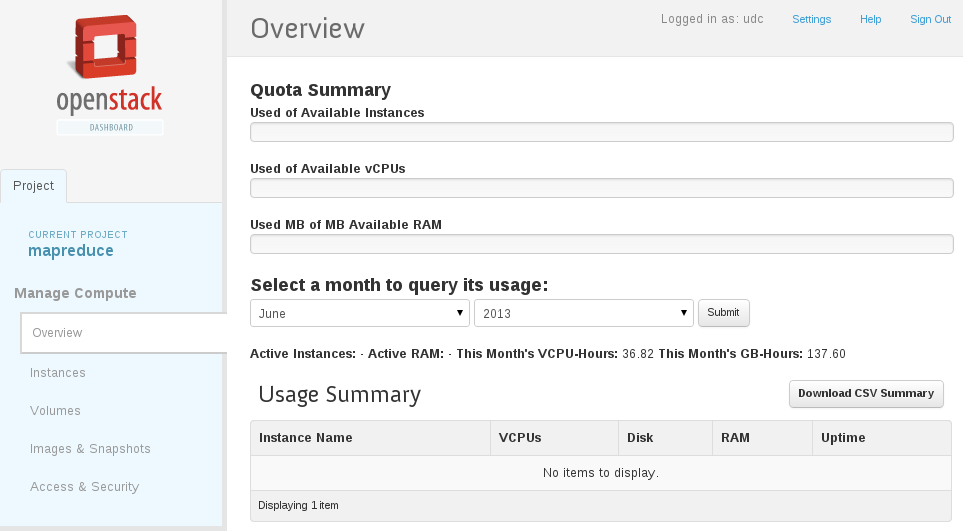
\includegraphics[width=0.99\textwidth]{imagenes/045.png}
\caption{OpenStack Folsom overview page}
\label{fig:homeos}
\end{center}
\end{figure}

At this point Django's development web server may be started to directly interact with qosh and check whether its installation succeeded --- figure \ref{fig:comandlsshell2} shows the command sequence to start the server. Again, a web browser shall be used to open \url{http://localhost:8000/albaproject/mapred}; then, qosh log in interface should load. Username and password are \emph{udc} again --- recall that user access is delegated entirely to OpenStack Keystone. Figure \ref{fig:comandosshell2} lists the commands that should be typed in a terminal.

\begin{figure}[tbp]
    \begin{center}
        \begin{tabular}{|l|}
            \hline
            \texttt{{\bf \$} cd quick-openstacked-hadoop/Alba/albaproject} \\
            \texttt{{\bf \$} python manage.py runserver} \\
            \hline
        \end{tabular}
        \caption{Command sequence II}
        \label{fig:comandosshell2}
    \end{center}
\end{figure}

\subsection{Testing a Work Flow for Hadoop}\label{subsec:flujohadoop}
\noindent Finally, to ensure every component is completely installed and configured, a real MapReduce work flow should be run in qosh. Input files for this test case might be downloaded from \url{https://code.google.com/p/quick-openstacked-hadoop/downloads/list} (\texttt{just\_imagine.tar.gz} and \texttt{bigtxt.tar.gz} --- zipped files containing plain-text files whose words will be counted --- and \texttt{wordcount.jar} --- package containing the classical word count MapReduce implementation.

Just after logging in, qosh's main page should load on screen. From there, \emph{Define Job} shall be clicked and the form that sets up the MapReduce job should appear. The fields should be filled in in a similar way as in figure \ref{fig:defmapredjob} before clicking \emph{launch} to begin the process. Once the job be completed the results may be downloaded from the \emph{Job History} page.

\begin{figure}[bp]
\begin{center}
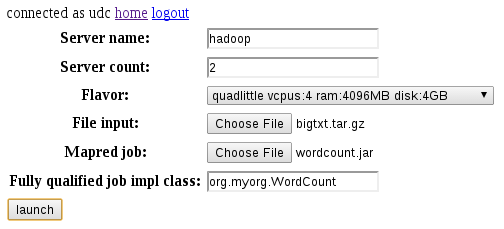
\includegraphics[width=0.90\textwidth]{imagenes/046.png}
\caption{MapReduce job definition}
\label{fig:defmapredjob}
\end{center}
\end{figure}

The image \ref{fig:mapredjobhistory} captures the \emph{Job History} page, and the image \ref{fig:mapredjobdetails} shows a capture detailing job \#56 from the \ref{Job Details} page.

\begin{figure}[tbp]
\begin{center}
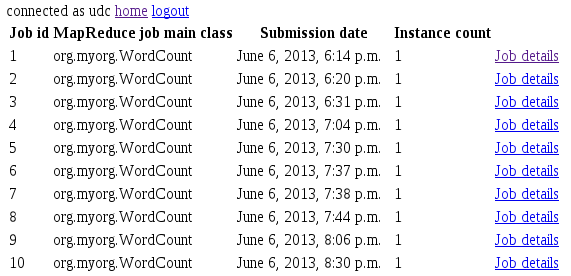
\includegraphics[width=0.99\textwidth]{imagenes/047.png}
\caption{MapReduce Job History}
\label{fig:mapredjobhistory}
\end{center}
\end{figure}

\begin{figure}[tbp]
\begin{center}
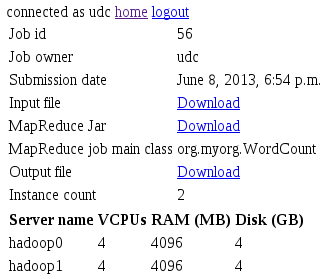
\includegraphics[width=0.60\textwidth]{imagenes/048.png}
\caption{Job \#56 details}
\label{fig:mapredjobdetails}
\end{center}
\end{figure}

\section{qosh's exploitation and maintenance}\label{sec:explotacionqosh}
\noindent To send MapReduce work flows into qosh, the operating procedure described in section \ref{subsec:flujohadoop} should be followed. Changing job options, cluster size, and main class may be accomplished by filling the form fields according to the user's needs.

By default qosh is configured to run in debug mode. This behavior may be easily modified by altering the flag \textbf{DEBUG} within \texttt{settings.py}. Furthermore, it should be noted that qosh will operate much faster when deployed to a production-level web server.

OpenStack Compute will keep a log in \texttt{/var/log/nova} that could be read should any issue appeared. By default, work flow computed results will be stored to \texttt{\$HOME/Public} which may be changed in \texttt{settings.py}, variable \textbf{MEDIA\_ROOT}.

%\cleardoublepage
%\chapter{Glossary of Terms}\label{cap:glosario}
\begin{description}
\item[ACPI] \texttt{Advanced Configuration and Power Interface}. A power management specification that makes hardware status information available to the operating system.
\item[AMD-V] \texttt{Advanced Micro Devices Virtualization}. Set of CPU extensions implemented by Advanced Micro Devices, Inc. to support Full Hardware Virtualization.
\item[API] \texttt{Application Programming Interface}. Protocol definition interface between two or more communicating entities. It specifies an abstract format by which collaborating entities can interchange information.
\item[APIC] \texttt{Advanced Programmable Interrupt Controller}. Family of interrupt controllers used to combine different interruption signal sources into one or more CPU lines, allowing for the assignment of priority levels to each kind of interruption.
\item[AWS] \texttt{Amazon Web Services}. Set of web services offered by Amazon Inc. that let a user exploit, remotely and on-demand, Amazon's computational infrastructure.
\item[CLI] \texttt{Command Line Interface}. Refers to every application whose main interface is the terminal or command line.
\item[CUDA] \texttt{Compute Unified Device Architecture}. Parallel computing platform and programming model devised at NVIDIA and implemented in its GPUs.
\item[DFS] \texttt{Distributed File System}. Any kind of file system stored over a network of computing devices and concurrently accessible by multiple users in different points.
\item[DHCP] \texttt{Dynamic Host Configuration Protocol}. Network protocol used to automatically and dynamically configure network access parameters.
\item[DNS] \texttt{Domain Name Server}. Name service that maps certain device information from one domain to another. It is typically used to locate resources in a network by translating their names to their IP addresses.
\item[Amazon EC2] \texttt{Elastic Compute Cloud}. Amazon, Inc.'s web service allowing for on-demand provisioning of computational infrastructure.
\item[EPT] \texttt{Extended Page Tables}. Intel's hardware virtualization system permitting a guest operating system to directly modify its own memory table pages, effectively requiring no VMM override to handle page misses.
\item[Hard coding] In Software Engineering, \emph{Hard coding} refers to the bad practice of including an input or configuration value within the source code that controls the application logic.
\item[Hash Function] An algorithm that associates a larger variable-length data space with a smaller fixed-length data space.
\item[HTTP] \texttt{HyperText Transfer Protocol}. Application protocol for distributed, collaborative, hypermedia information systems. HTTP is the foundation of data communication for the World Wide Web.
\item[HVM] \texttt{Hardware Virtual Machine}. Virtualization approach by which a modified CPU is able to create a virtual domain for applications to exploit infrastructure resources with reduced penalty on performance. Also called \emph{Native Virtualization}.
\item[iptables] Administrative tool and associated Linux service that allows configuring the routing tables provided by the kernel firewall and the chains and rules it stores.
\item[IT] \texttt{Information Technology}. It comprises any concept related to information and the technology to handle it, like networks, hardware, software, the Internet, as well as the people working with these technologies.
\item[JRE] \texttt{Java Runtime Environment}. Environment that need be installed in any computer requiring the execution of Java applications.
\item[KVM] \texttt{Kernel-based Virtual Machine}. Full Virtualization solution for the Linux kernel that turns it into a hypervisor. KVM requires a processor with hardware virtualization extensions.
\item[LVM] \texttt{Logical Volume Manager}. Tool set that allows a user to define an storage abstraction layer on top of conventional persistence that is more flexible than conventional partitioning schemes.
\item[MMU] \texttt{Memory Management Unit}. Hardware device, on-die in modern CPU architectures, that handles access to main memory.
\item[NAS] \texttt{Network Attached Storage}. Storage device that is attached to a preexisting network to increase the shared storage space.
\item[NAT] \texttt{Network Address Translation}. Process by which some networking devices rewrite the source and/or destination fields in telecommunications within a network segment. It is used as a means to limit the number of issued network addresses and to conceal the identity of devices behind the NAT.
\item[NFS] \texttt{Network File System}. A file system developed by Sun Microsystems, Inc. implementing client/server model that allows users to access files across a network and treat them as if they resided in a local file directory.
\item[NTP] \texttt{Network Time Protocol}. It is a networking protocol for clock synchronization between computer systems over packet-switched, variable-latency data networks.
\item[OCCI] \texttt{Open Cloud Computing Interface}. A set of specifications delivered through the Open Grid Forum, for cloud computing service providers to offer their services defining a unified interface.
\item[QCOW2] \texttt{QEMU Copy On Write 2}. Optimization strategy by which a storage device will delay the allocation of storage space until it is actually needed.
\item[QEMU] \texttt{Quick EMUlator}. Free and open source hosted hypervisor that performs hardware virtualization.
\item[RAID] \texttt{Redudant Array of Independent Disks}. It is a data storage virtualization technology that combines multiple disk drive components into a logical unit for the purposes of data redundancy or performance improvement.
\item[REST] \texttt{Representational State Tranfer}. Client/server architectural style that defines a simple, stateless, cacheable, interface-uniform protocol used to handle resource representation in distributed systems.
\item[RPC] \texttt{Remote Procedure Call}. An inter-process communication that allows a computer program to cause a subroutine or procedure to execute in another address space (commonly on another computer on a shared network) without the programmer explicitly coding the details for this remote interaction.
\item[RPM] \texttt{RPM Package Manager}. A package management system for the Red Hat Enterprise Linux and derivatives.
\item[rsync] Is a file synchronization and file transfer program for Unix-like systems that minimizes network data transfer by using a form of delta encoding called the rsync algorithm. rsync can compress the data transferred further using zlib compression, and SSH or stunnel can be used to encrypt the transfer.
\item[Amazon S3] \texttt{Simple Storage Service}. Scalable, safe, fast and inexpensive storage service consumed through the Internet and provided by Amazon, Inc.
\item[SAN] \texttt{Storage Area Network}. It is a dedicated network that provides access to consolidated, block level data storage.
\item[Sandbox] In the context of software development and revision control, it is a testing environment that isolates untested code changes and outright experimentation from the production environment or repository respectively.
\item[SELinux] \texttt{Security-Enhanced Linux}. A Linux kernel security module that provides a mechanism for supporting access control security policies, including United States Department of Defense-style mandatory access controls (\emph{MAC}).
\item[SPOF] \texttt{Single Point Of Failure}. In Systems Engineering it is the point of the architecture that if it failed it would prevent the whole system from functioning.
\item[Amazon SQS] \texttt{Simple Queue Service}. Queue service provided by Amazon, Inc. to handle asynchronous message passing between EC2 instances.
\item[SSH] \texttt{Secure SHell}. A cryptographic network protocol for secure data communication, remote command-line login, remote command execution, and other secure network services between two networked computers.
\item[sudoers] The file in a *nix system that specifies which users can execute commands as if they were the root user.
\item[VMM] \texttt{Virtual Machine Manager}. A management solution for the virtualized data center. It can be used to configure the virtualization host, networking, and storage resources, in order to create and deploy virtual machines and services to private clouds.
\item[VT-x] Intel, Inc.'s CPU extension set allowing for full hardware virtualization.
\item[yum] \texttt{Yellowdog Updater Modified}. An open source command-line package-management utility for Linux operating systems using the RPM Package Manager.
\end{description}


%\cleardoublepage
%\nocite{*}
%\bibliography{biblio}
%\markboth{Bibliografia}{Bibliografia}
%\addcontentsline{toc}{chapter}{Bibliografia}

\end{document}

